\documentclass[10pt]{article}\usepackage[]{graphicx}\usepackage[]{xcolor}
% maxwidth is the original width if it is less than linewidth
% otherwise use linewidth (to make sure the graphics do not exceed the margin)
\makeatletter
\def\maxwidth{ %
  \ifdim\Gin@nat@width>\linewidth
    \linewidth
  \else
    \Gin@nat@width
  \fi
}
\makeatother

\definecolor{fgcolor}{rgb}{0.345, 0.345, 0.345}
\newcommand{\hlnum}[1]{\textcolor[rgb]{0.686,0.059,0.569}{#1}}%
\newcommand{\hlsng}[1]{\textcolor[rgb]{0.192,0.494,0.8}{#1}}%
\newcommand{\hlcom}[1]{\textcolor[rgb]{0.678,0.584,0.686}{\textit{#1}}}%
\newcommand{\hlopt}[1]{\textcolor[rgb]{0,0,0}{#1}}%
\newcommand{\hldef}[1]{\textcolor[rgb]{0.345,0.345,0.345}{#1}}%
\newcommand{\hlkwa}[1]{\textcolor[rgb]{0.161,0.373,0.58}{\textbf{#1}}}%
\newcommand{\hlkwb}[1]{\textcolor[rgb]{0.69,0.353,0.396}{#1}}%
\newcommand{\hlkwc}[1]{\textcolor[rgb]{0.333,0.667,0.333}{#1}}%
\newcommand{\hlkwd}[1]{\textcolor[rgb]{0.737,0.353,0.396}{\textbf{#1}}}%
\let\hlipl\hlkwb

\usepackage{framed}
\makeatletter
\newenvironment{kframe}{%
 \def\at@end@of@kframe{}%
 \ifinner\ifhmode%
  \def\at@end@of@kframe{\end{minipage}}%
  \begin{minipage}{\columnwidth}%
 \fi\fi%
 \def\FrameCommand##1{\hskip\@totalleftmargin \hskip-\fboxsep
 \colorbox{shadecolor}{##1}\hskip-\fboxsep
     % There is no \\@totalrightmargin, so:
     \hskip-\linewidth \hskip-\@totalleftmargin \hskip\columnwidth}%
 \MakeFramed {\advance\hsize-\width
   \@totalleftmargin\z@ \linewidth\hsize
   \@setminipage}}%
 {\par\unskip\endMakeFramed%
 \at@end@of@kframe}
\makeatother

\definecolor{shadecolor}{rgb}{.97, .97, .97}
\definecolor{messagecolor}{rgb}{0, 0, 0}
\definecolor{warningcolor}{rgb}{1, 0, 1}
\definecolor{errorcolor}{rgb}{1, 0, 0}
\newenvironment{knitrout}{}{} % an empty environment to be redefined in TeX

\usepackage{alltt}
\usepackage[left=1in,right=1in,top=1in,bottom=1in]{geometry}
\usepackage{amsmath}
\usepackage{hyperref}
%\SweaveOpts[concordance=TRUE]
\IfFileExists{upquote.sty}{\usepackage{upquote}}{}
\begin{document}

\begin{titlepage}
    \centering
    
    { \Huge \textbf{Final Project Report Draft 2} \par} 
    \vspace{5mm}
    { \huge \textbf{Motor vehicle colisions in NYC} \par} 
    \vspace{3mm}
    { \Large Group 1 (STAT 605 - S1)\par}  
    
    \vspace{5mm}
    \begin{center}
    \line(1,0){425}
    \end{center}
    
    \vspace{5mm}

    \vspace{15mm}
    { \large Authors: \par }
      \vspace{3mm}
    { \Large \textbf{Astha Singh} - \texttt{as677@rice.edu} \par}
    { \Large \textbf{Franco Bosetti} - \texttt{fb57@rice.edu}\par}
    { \Large \textbf{Louis Clarke} - \texttt{lc160@rice.edu}\par}
    { \Large \textbf{Lindsey Russ} - \texttt{ltr1@rice.edu}\par}
    
    
    \vspace{5mm}
    
    \vspace{5mm}

\end{titlepage}

\newpage


\tableofcontents

\newpage

\section{Introduction}

Motor vehicle collisions are a major concern in major populated urban areas like New York City (NYC), where millions of people use diverse transportation systems every day. Understanding these incidents through data analysis can help us identify patterns and make safety improvements. At the same time, social media platforms such as Twitter have become spaces where people share their real-time information about traffic incidents and congestion. This project will analyze NYC motor vehicle collision data alongside Twitter traffic discussions, while also incorporating roadway speed limit data and detailed vehicle-level records to examine how roadway conditions, vehicle characteristics, and public reporting intersect with officially documented traffic incidents.

\section{Dataset Description}
Primary Dataset: NYC Motor Vehicle Collisions 

(\url{https://data.cityofnewyork.us/Public-Safety/Motor-Vehicle-Collisions-Crashes/h9gi-nx95/about_data})

Our primary dataset contains police-reported motor vehicle collision records from New York City, maintained by the NYPD through their TrafficStat initiative. The dataset includes 2.21 million collision records with 29 variables.


Source: NYC OpenData (2025)


Key variables include:
\begin{itemize}
  \item Location \& Time: Borough, coordinates (latitude \& longitude), street names, zip codes, crash date/time
  \item Casualties: Injuries and fatalities by category (pedestrians, cyclists, motorists)
  \item Contributing Factors: Up to five causal factors per collision
  \item Vehicle Types: Vehicle type classifications (ATV, bicycle, car/SUV, e-bike, e-scooter, truck/bus, motorcycle, other) for each vehicle involved
\end{itemize}


Preprocessing: We prepared the dataset for analysis by converting crash dates to a standard date format, organizing borough names as categorical variables, and creating additional time-based variables to explore patterns across years and months. 

Secondary Dataset: Twitter Traffic Classifications (\url{https://data.mendeley.com/datasets/c3xvj5snvv/1})

Our secondary dataset contains classified tweets collected from Twitter's API, with each tweet categorized by its traffic-related content.


Source: Research dataset by Sina Dabiri (2018)


Variables include:
\begin{itemize}
  \item Tweet ID
  \item Classification label: 
  \item Non-Traffic (Class 0): General tweets unrelated to traffic
  \item Traffic Incident (Class 1): Reports of crashes, breakdowns, road closures
  \item Traffic Conditions (Class 2): Congestion reports, traffic advisories, flow conditions
  \item Tweet text content
\end{itemize}


Preprocessing: We combined the training and test datasets into one dataset since we don’t plan to run a classification model. We renamed variables for clarity and ensured consistency in column naming. Our next step is cleaning the dataset and the text data to prepare for sentiment analysis and linking patterns with NYC collision data.

Tertiary Dataset: NYC Speed Limits (\url{https://data.cityofnewyork.us/Transportation/VZV_Speed-Limits/5mad-ntua/about_data}) 

Our tertiary dataset provided posted speed limits across NYC streets, maintained under the Vision Zero initiative. This dataset will allow us to explore whether high-speed areas correlate with higher accident frequency and severity.


Source: NYC OpenData (2025)


Variables include:
\begin{itemize}
  \item Segment Geometry: street segment represented as geographic coordinates (longitude \& latitude)
  \item Posted Speed Limit: legal speed limit value for each street segment
  \item Street Name
  \item Borough
\end{itemize}

Preprocessing: We extracted latitude and longitude from the geometric strings and rounded them to 4 decimals to match with collision coordinates. This allowed us to link crash locations to nearby street segments. We also filtered roads with speed limits above 40 mph to compare crashes on high-speed vs. lower-speed roads. 

Quaternary Dataset: Motor Vehicle Collisions - Vehicles (\url{https://data.cityofnewyork.us/Public-Safety/Motor-Vehicle-Collisions-Vehicles/bm4k-52h4/about_data}) 

Our quaternary dataset gives vehicle-level details for each crash in NYC. Unlike the primary collisions dataset, where each row represents a crash, here each row represents a single vehicle involved. This will give us insights into how vehicle type, driver demographics, and pre-crash behavior contribute to accidents.

Source: NYC OpenData (2025)


Variables include:
\begin{itemize}
  \item Collision information 
  \item Vehicle details 
  \item Driver information
  \item Crash circumstances 
  \item Contributing factors 
\end{itemize}

Preprocessing: We plan to link this dataset with the primary collisions dataset using the 'collision\_id' key. This will also expand our crash-level analysis with vehicle-level and driver-level details, such as identifying trends in which vehicle types are most frequently involved in accidents and which driver factors contribute most to severe outcomes.  

\newpage


\section{Data Preparation}

Prepare the data for processing:



\begin{knitrout}
\definecolor{shadecolor}{rgb}{0.969, 0.969, 0.969}\color{fgcolor}\begin{kframe}
\begin{alltt}
\hldef{nyc} \hlkwb{<-} \hlkwd{read.csv}\hldef{(}\hlkwc{file} \hldef{=} \hlsng{"data/Motor_Vehicle_Collisions_-_Crashes.csv"}\hldef{)}
\hldef{nyc}\hlopt{$}\hldef{CRASH.DATE} \hlkwb{<-} \hlkwd{as.Date}\hldef{(nyc}\hlopt{$}\hldef{CRASH.DATE,} \hlkwc{format} \hldef{=} \hlsng{"%m/%d/%Y"}\hldef{)}
\hldef{nyc}\hlopt{$}\hldef{BOROUGH} \hlkwb{<-} \hlkwd{factor}\hldef{(nyc}\hlopt{$}\hldef{BOROUGH)}
\hldef{nyc}\hlopt{$}\hldef{YEAR_MONTH} \hlkwb{<-} \hlkwd{format}\hldef{(nyc}\hlopt{$}\hldef{CRASH.DATE,} \hlsng{"%Y-%m"}\hldef{)}
\hldef{nyc}\hlopt{$}\hldef{YEAR} \hlkwb{<-} \hlkwd{format}\hldef{(nyc}\hlopt{$}\hldef{CRASH.DATE,} \hlsng{"%Y"}\hldef{)}
\hldef{nyc_longs} \hlkwb{<-} \hldef{nyc}\hlopt{$}\hldef{LONGITUDE}
\hldef{nyc_lats} \hlkwb{<-} \hldef{nyc}\hlopt{$}\hldef{LATITUDE}
\hldef{nyc}\hlopt{$}\hldef{round_location} \hlkwb{<-} \hlkwd{paste}\hldef{(}\hlsng{"("}\hldef{,} \hlkwd{round}\hldef{(nyc_lats,} \hlkwc{digits} \hldef{=} \hlnum{4}\hldef{),} \hlsng{", "}\hldef{,}
                            \hlkwd{round}\hldef{(nyc_longs,} \hlkwc{digits} \hldef{=} \hlnum{4}\hldef{),} \hlsng{")"}\hldef{,} \hlkwc{sep} \hldef{=} \hlsng{""}\hldef{)}
\hldef{nyc}\hlopt{$}\hldef{HOUR} \hlkwb{<-} \hlkwd{as.numeric}\hldef{(}\hlkwd{sub}\hldef{(}\hlsng{"\textbackslash{}\textbackslash{}:.*"}\hldef{,} \hlsng{""}\hldef{, nyc}\hlopt{$}\hldef{CRASH.TIME))}
\end{alltt}
\end{kframe}
\end{knitrout}

\subsection{Secondary Datasets}
While the New York Collisions dataset provides many useful columns on which to perform analysis, more insight can be gained when considering other forms of data. Below we import these auxillary datasets:

\begin{knitrout}
\definecolor{shadecolor}{rgb}{0.969, 0.969, 0.969}\color{fgcolor}\begin{kframe}
\begin{alltt}
\hldef{twitter_train} \hlkwb{<-} \hlkwd{read.csv}\hldef{(}\hlsng{"data/1_TrainingSet_3Class.csv"}\hldef{,} \hlkwc{header}\hldef{=}\hlnum{FALSE}\hldef{)}
\hldef{twitter_test} \hlkwb{<-} \hlkwd{read.csv}\hldef{(}\hlsng{"data/1_TestSet_3Class.csv"}\hldef{,} \hlkwc{header}\hldef{=}\hlnum{FALSE}\hldef{)}

\hlcom{# add headers}
\hlkwd{names}\hldef{(twitter_train)} \hlkwb{<-} \hlkwd{c}\hldef{(}\hlsng{"class"}\hldef{,} \hlsng{"tweet_id"}\hldef{,} \hlsng{"tweet_text"}\hldef{)}
\hlkwd{names}\hldef{(twitter_test)} \hlkwb{<-} \hlkwd{c}\hldef{(}\hlsng{"class"}\hldef{,} \hlsng{"tweet_id"}\hldef{,} \hlsng{"tweet_text"}\hldef{)}

\hlcom{# Combine }
\hldef{twitter} \hlkwb{<-} \hlkwd{rbind}\hldef{(twitter_train, twitter_test)}
\end{alltt}
\end{kframe}
\end{knitrout}


The VZV dataset on speed limits contains a map of city speed limits. Each speed limit is attached to a street or section of a street, specified by a sequence of coordinates. From this, spatial analysis can be performed related collisions to repsective speed limits.
\begin{knitrout}
\definecolor{shadecolor}{rgb}{0.969, 0.969, 0.969}\color{fgcolor}\begin{kframe}
\begin{alltt}
\hldef{sp_limits} \hlkwb{<-} \hlkwd{read.csv}\hldef{(}\hlsng{"data/VZV_Speed_Limits_20251002.csv"}\hldef{)}

\hlcom{# Format the sp_limits latitude and longitude}
\hldef{splitted} \hlkwb{<-} \hlkwd{strsplit}\hldef{(sp_limits}\hlopt{$}\hldef{the_geom,} \hlsng{" "}\hldef{)}
\hldef{lats} \hlkwb{<-} \hlkwd{as.numeric}\hldef{(}\hlkwd{lapply}\hldef{(splitted,} \hlkwa{function}\hldef{(}\hlkwc{x}\hldef{)} \hlkwd{substr}\hldef{(x[}\hlnum{3}\hldef{],} \hlnum{1}\hldef{,} \hlkwd{nchar}\hldef{(x[}\hlnum{3}\hldef{])}\hlopt{-}\hlnum{1}\hldef{)))}
\hldef{longs} \hlkwb{<-} \hlkwd{as.numeric}\hldef{(}\hlkwd{lapply}\hldef{(splitted,} \hlkwa{function}\hldef{(}\hlkwc{x}\hldef{)} \hlkwd{substr}\hldef{(x[}\hlnum{2}\hldef{],} \hlnum{3}\hldef{,} \hlkwd{nchar}\hldef{(x[}\hlnum{3}\hldef{]))))}
\hldef{sp_limits}\hlopt{$}\hldef{latitude} \hlkwb{<-} \hldef{lats}
\hldef{sp_limits}\hlopt{$}\hldef{longitude} \hlkwb{<-} \hldef{longs}
\hldef{sp_limits}\hlopt{$}\hldef{location} \hlkwb{<-} \hlkwd{paste}\hldef{(}\hlsng{"("}\hldef{,} \hlkwd{round}\hldef{(lats,} \hlkwc{digits} \hldef{=} \hlnum{4}\hldef{),} \hlsng{", "}\hldef{,}
                            \hlkwd{round}\hldef{(longs,} \hlkwc{digits} \hldef{=} \hlnum{4}\hldef{),} \hlsng{")"}\hldef{,} \hlkwc{sep} \hldef{=} \hlsng{""}\hldef{)}

\hlcom{# Add a rounded location value to the nyc dataset}
\hldef{has_long_lat} \hlkwb{<-} \hldef{nyc[}\hlopt{!}\hlkwd{is.na}\hldef{(nyc}\hlopt{$}\hldef{LONGITUDE)} \hlopt{& !}\hlkwd{is.na}\hldef{(nyc}\hlopt{$}\hldef{LATITUDE),]}
\hldef{nyc_longs} \hlkwb{<-} \hldef{has_long_lat}\hlopt{$}\hldef{LONGITUDE}
\hldef{nyc_lats} \hlkwb{<-} \hldef{has_long_lat}\hlopt{$}\hldef{LATITUDE}
\hldef{has_long_lat}\hlopt{$}\hldef{round_location} \hlkwb{<-} \hlkwd{paste}\hldef{(}\hlsng{"("}\hldef{,} \hlkwd{round}\hldef{(nyc_lats,} \hlkwc{digits} \hldef{=} \hlnum{4}\hldef{),} \hlsng{", "}\hldef{,}
                                     \hlkwd{round}\hldef{(nyc_longs,} \hlkwc{digits} \hldef{=} \hlnum{4}\hldef{),} \hlsng{")"}\hldef{,}
                                     \hlkwc{sep} \hldef{=} \hlsng{""}\hldef{)}
\end{alltt}
\end{kframe}
\end{knitrout}


The Motor Vehicle Collisions vehicle table contains details on each vehicle involved in a collision. Each row represents a particular vehicle with certain attributes. The collision ID of the main dataset is also present in this dataset, although values are no longer unique as multiple vehicles can contribute to one collision.
\begin{knitrout}
\definecolor{shadecolor}{rgb}{0.969, 0.969, 0.969}\color{fgcolor}\begin{kframe}
\begin{alltt}
\hldef{nyv} \hlkwb{<-} \hlkwd{read.csv}\hldef{(}\hlkwc{file} \hldef{=} \hlsng{"data/Motor_Vehicle_Collisions_-_Vehicles_20251002.csv"}\hldef{)}
\hldef{nyv}\hlopt{$}\hldef{CRASH_DATE} \hlkwb{<-} \hlkwd{as.Date}\hldef{(nyv}\hlopt{$}\hldef{CRASH_DATE,} \hlkwc{format} \hldef{=} \hlsng{"%m/%d/%Y"}\hldef{)}
\hldef{nyv}\hlopt{$}\hldef{YEAR} \hlkwb{<-} \hlkwd{as.numeric}\hldef{(}\hlkwd{format}\hldef{(nyv}\hlopt{$}\hldef{CRASH_DATE,} \hlsng{"%Y"}\hldef{))}

\hldef{veh_per_col} \hlkwb{<-} \hlkwd{tapply}\hldef{(nyv}\hlopt{$}\hldef{COLLISION_ID, nyv}\hlopt{$}\hldef{COLLISION_ID, length)}
\hldef{nyc}\hlopt{$}\hldef{VEHICLE_COUNT} \hlkwb{<-} \hldef{veh_per_col[}\hlkwd{as.character}\hldef{(nyc}\hlopt{$}\hldef{COLLISION_ID)]}

\hlcom{#rows where vehicle occupants is not NA, }
\hlcom{#not 0 and not above 60 (capacity of New York Bus)}
\hldef{ex_pas_move} \hlkwb{<-} \hldef{(}\hlopt{!}\hlkwd{is.na}\hldef{(nyv}\hlopt{$}\hldef{VEHICLE_OCCUPANTS))}\hlopt{&}\hldef{(nyv}\hlopt{$}\hldef{VEHICLE_OCCUPANTS} \hlopt \hlnum{1}\hlopt{:}\hlnum{60}\hldef{)}
\hldef{pass_per_veh} \hlkwb{<-} \hlkwd{tapply}\hldef{(nyv}\hlopt{$}\hldef{VEHICLE_OCCUPANTS[ex_pas_move],}
                       \hldef{nyv}\hlopt{$}\hldef{COLLISION_ID[ex_pas_move],}
                       \hldef{mean)}
\hldef{nyc}\hlopt{$}\hldef{AV_PASSENGERS} \hlkwb{<-} \hldef{pass_per_veh[}\hlkwd{as.character}\hldef{(nyc}\hlopt{$}\hldef{COLLISION_ID)]}

\hlcom{#Select only vehicle year models from 1920-2025 to clean the data}
\hldef{ex_veh_year} \hlkwb{<-} \hldef{(}\hlopt{!}\hlkwd{is.na}\hldef{(nyv}\hlopt{$}\hldef{VEHICLE_YEAR))}\hlopt{&}
               \hldef{(nyv}\hlopt{$}\hldef{VEHICLE_YEAR} \hlopt \hlnum{1920}\hlopt{:}\hlnum{2025}\hldef{)} \hlopt{&}
               \hldef{(nyv}\hlopt{$}\hldef{VEHICLE_YEAR} \hlopt{<=} \hldef{nyv}\hlopt{$}\hldef{YEAR)}

\hldef{av_car_made} \hlkwb{<-} \hlkwd{tapply}\hldef{(nyv}\hlopt{$}\hldef{VEHICLE_YEAR[ex_veh_year],}
                      \hldef{nyv}\hlopt{$}\hldef{COLLISION_ID[ex_veh_year],}
                      \hldef{mean)}
\hldef{nyc}\hlopt{$}\hldef{AV_VEH_YEAR} \hlkwb{<-} \hldef{av_car_made[}\hlkwd{as.character}\hldef{(nyc}\hlopt{$}\hldef{COLLISION_ID)]}

\hlcom{#Add average vehicle age column.}
\hlcom{#Note that vehicles year sometimes given as year rounded up.}
\hldef{nyc}\hlopt{$}\hldef{AV_VEH_AGE} \hlkwb{<-}  \hlkwd{as.numeric}\hldef{(nyc}\hlopt{$}\hldef{YEAR)} \hlopt{-} \hldef{nyc}\hlopt{$}\hldef{AV_VEH_YEAR}
\end{alltt}
\end{kframe}
\end{knitrout}

\section{Visualizations}

\subsection{Vehicle Collisions over Time}
By grouping the collisions into each month in which they occured, we can plot a line graph showing the number of collisions over the past 13 years.
\begin{knitrout}
\definecolor{shadecolor}{rgb}{0.969, 0.969, 0.969}\color{fgcolor}\begin{kframe}
\begin{alltt}
\hldef{monthly_counts} \hlkwb{<-} \hlkwd{table}\hldef{(nyc}\hlopt{$}\hldef{YEAR_MONTH)}
\hldef{months} \hlkwb{<-} \hlkwd{names}\hldef{(monthly_counts)}
\hldef{colspermonth} \hlkwb{<-} \hlkwd{as.numeric}\hldef{(monthly_counts)}
\hldef{plot_months} \hlkwb{<-} \hlkwd{as.Date}\hldef{(}\hlkwd{paste0}\hldef{(months,} \hlsng{"-01"}\hldef{))}
\hlkwd{plot}\hldef{(plot_months, colspermonth,}
     \hlkwc{main}\hldef{=}\hlsng{"Number of Monthly Vehicle Collisions in New York City"}\hldef{,}
     \hlkwc{type}\hldef{=}\hlsng{"o"}\hldef{,}
     \hlkwc{pch}\hldef{=}\hlnum{20}\hldef{,}
     \hlkwc{xlab}\hldef{=}\hlsng{"Month"}\hldef{,}
     \hlkwc{ylab}\hldef{=}\hlsng{"Number of Collisions"}\hldef{,}
     \hlkwc{xaxt}\hldef{=}\hlsng{"n"}\hldef{,}
     \hlkwc{yaxt}\hldef{=}\hlsng{"n"}\hldef{,}
     \hlkwc{xaxs}\hldef{=}\hlsng{"i"}\hldef{,}
     \hlkwc{yaxs}\hldef{=}\hlsng{"i"}\hldef{,}
     \hlkwc{ylim}\hldef{=}\hlkwd{c}\hldef{(}\hlnum{0}\hldef{,}\hlkwd{max}\hldef{(colspermonth)}\hlopt{+}\hlnum{1000}\hldef{))}


\hldef{xticks} \hlkwb{<-} \hlkwd{seq}\hldef{(}\hlkwd{min}\hldef{(plot_months),} \hlkwd{max}\hldef{(plot_months)}\hlopt{+}\hlnum{365}\hldef{,} \hlkwc{by} \hldef{=} \hlsng{"6 months"}\hldef{)}
\hlkwd{axis.Date}\hldef{(}\hlnum{1}\hldef{,} \hlkwc{at} \hldef{= xticks,}
          \hlkwc{format} \hldef{=} \hlsng{"%b\textbackslash{}n%Y"}\hldef{,} \hlkwc{cex.axis} \hldef{=} \hlnum{0.6}\hldef{)}
\hlkwd{axis}\hldef{(}\hlnum{2}\hldef{,} \hlkwc{at} \hldef{=} \hlkwd{seq}\hldef{(}\hlnum{0}\hldef{,} \hlkwd{max}\hldef{(colspermonth)}\hlopt{+}\hlnum{1000}\hldef{,} \hlkwc{by} \hldef{=} \hlnum{1000}\hldef{),} \hlkwc{cex.axis} \hldef{=} \hlnum{0.7}\hldef{,} \hlkwc{las}\hldef{=}\hlnum{1}\hldef{)}
\hlkwd{abline}\hldef{(}\hlkwc{v} \hldef{= xticks,} \hlkwc{col} \hldef{=} \hlsng{"gray"}\hldef{,} \hlkwc{lty} \hldef{=} \hlsng{"dotted"}\hldef{)}
\end{alltt}
\end{kframe}
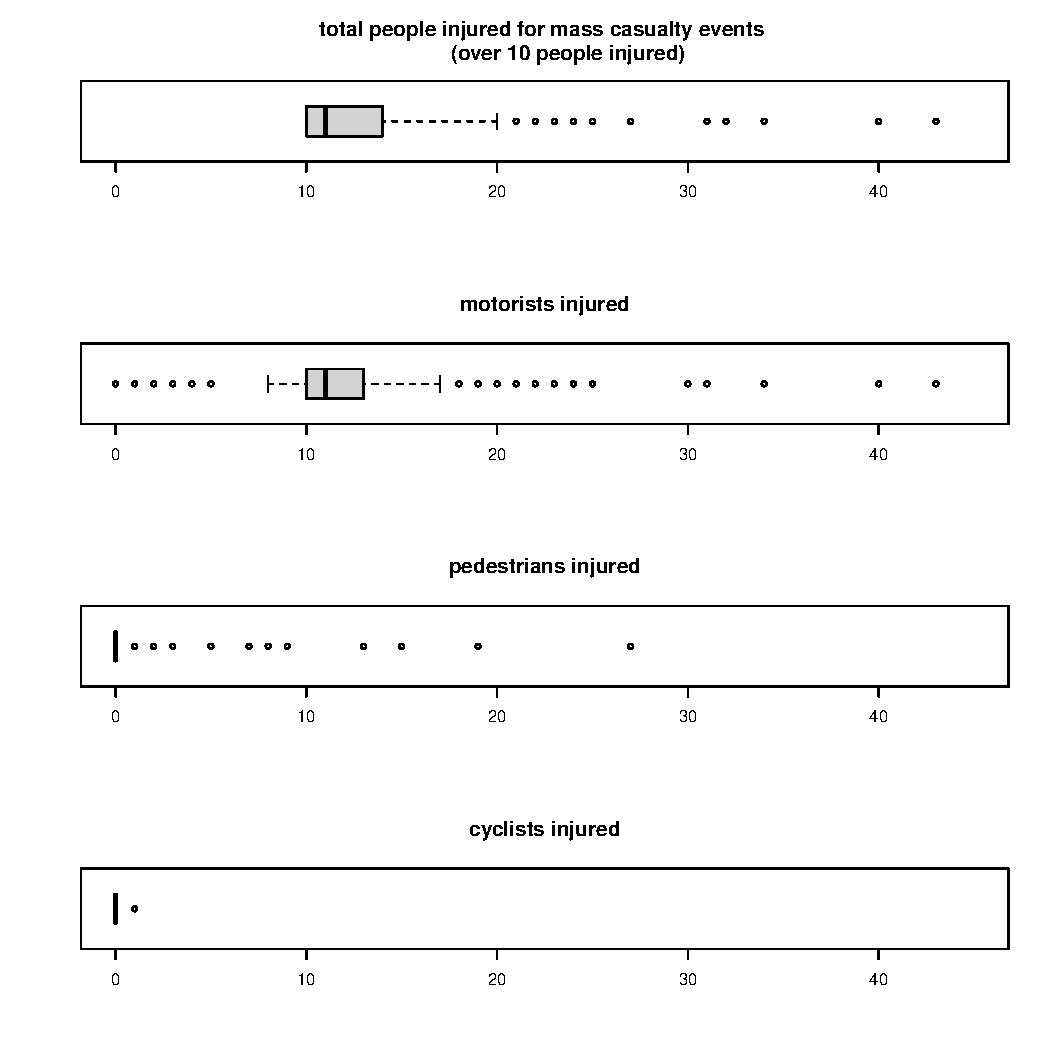
\includegraphics[width=\maxwidth]{figure/unnamed-chunk-6-1} 
\end{knitrout}
A notable trend is the sudden drop in collisions at the beginning of 2020. This is clearly due to the Covid-19 pandemic, which limited the time people spent outside their homes. What is more notable is how the number of collisions seems to even out to a much lower level than pre-pandemic. More research is needed into why we see this pattern.
\\ \\
Next, we explore the number of collisions over time within each borough. Note that a large quantity of entries from the dataset do not have a location attached, so those results are not considered for this analysis.
\begin{knitrout}
\definecolor{shadecolor}{rgb}{0.969, 0.969, 0.969}\color{fgcolor}\begin{kframe}
\begin{alltt}
\hldef{borough} \hlkwb{<-} \hlkwd{levels}\hldef{(nyc}\hlopt{$}\hldef{BOROUGH)}
\hldef{borough} \hlkwb{<-} \hldef{borough[borough} \hlopt{!=} \hlsng{""}\hldef{]}
\hldef{colors} \hlkwb{=} \hlkwd{c}\hldef{(}\hlsng{"red"}\hldef{,} \hlsng{"blue"}\hldef{,} \hlsng{"darkgreen"}\hldef{,} \hlsng{"purple"}\hldef{,} \hlsng{"orange"}\hldef{)}
\hldef{plot_months} \hlkwb{<-} \hlkwd{list}\hldef{()}
\hldef{colspermonth} \hlkwb{<-} \hlkwd{list}\hldef{()}
\hlkwa{for} \hldef{(b} \hlkwa{in} \hldef{borough)\{}
  \hldef{monthly_counts} \hlkwb{<-} \hlkwd{table}\hldef{(nyc}\hlopt{$}\hldef{YEAR_MONTH[nyc}\hlopt{$}\hldef{BOROUGH}\hlopt{==}\hldef{b])}
  \hldef{months} \hlkwb{<-} \hlkwd{names}\hldef{(monthly_counts)}
  \hldef{colspermonth[[b]]} \hlkwb{<-} \hlkwd{as.numeric}\hldef{(monthly_counts)}
  \hldef{plot_months[[b]]} \hlkwb{<-} \hlkwd{as.Date}\hldef{(}\hlkwd{paste0}\hldef{(months,} \hlsng{"-01"}\hldef{))}
\hldef{\}}

\hldef{max_col} \hlkwb{<-} \hlkwd{max}\hldef{(}\hlkwd{sapply}\hldef{(colspermonth, max))}
\hldef{min_dat} \hlkwb{<-} \hlkwd{as.Date}\hldef{(}\hlkwd{min}\hldef{(}\hlkwd{sapply}\hldef{(plot_months,min)))}
\hldef{max_dat} \hlkwb{<-} \hlkwd{as.Date}\hldef{(}\hlkwd{max}\hldef{(}\hlkwd{sapply}\hldef{(plot_months,max)))}

\hlkwd{plot}\hldef{(plot_months[[}\hlnum{1}\hldef{]], colspermonth[[}\hlnum{1}\hldef{]],}
     \hlkwc{main}\hldef{=}\hlsng{"Number of Monthly Vehicle Collisions in New York City"}\hldef{,}
     \hlkwc{type}\hldef{=}\hlsng{"l"}\hldef{,}
     \hlkwc{pch}\hldef{=}\hlnum{20}\hldef{,}
     \hlkwc{col}\hldef{= colors[}\hlnum{1}\hldef{],}
     \hlkwc{xlab}\hldef{=}\hlsng{"Month"}\hldef{,}
     \hlkwc{ylab}\hldef{=}\hlsng{"Number of Collisions"}\hldef{,}
     \hlkwc{xaxt}\hldef{=}\hlsng{"n"}\hldef{,}
     \hlkwc{yaxt}\hldef{=}\hlsng{"n"}\hldef{,}
     \hlkwc{xaxs}\hldef{=}\hlsng{"i"}\hldef{,}
     \hlkwc{yaxs}\hldef{=}\hlsng{"i"}\hldef{,}
     \hlkwc{ylim}\hldef{=}\hlkwd{c}\hldef{(}\hlnum{0}\hldef{,max_col}\hlopt{+}\hlnum{500}\hldef{))}

\hlkwa{for} \hldef{(i} \hlkwa{in} \hlnum{2}\hlopt{:}\hldef{(}\hlkwd{length}\hldef{(borough)))\{}
  \hlkwd{lines}\hldef{(plot_months[[i]], colspermonth[[i]],} \hlkwc{type}\hldef{=}\hlsng{"l"}\hldef{,} \hlkwc{pch}\hldef{=}\hlnum{20}\hldef{,} \hlkwc{col}\hldef{=colors[i])}
\hldef{\}}

\hlkwd{legend}\hldef{(}\hlsng{"topright"}\hldef{,}
       \hlkwc{legend} \hldef{= borough,}
       \hlkwc{col} \hldef{= colors,}
       \hlkwc{lty} \hldef{=} \hlnum{1}\hldef{)}


\hldef{xticks} \hlkwb{<-} \hlkwd{seq}\hldef{(min_dat, max_dat}\hlopt{+}\hlnum{365}\hldef{,} \hlkwc{by} \hldef{=} \hlsng{"6 months"}\hldef{)}
\hlkwd{axis.Date}\hldef{(}\hlnum{1}\hldef{,} \hlkwc{at} \hldef{= xticks,}
          \hlkwc{format} \hldef{=} \hlsng{"%b\textbackslash{}n%Y"}\hldef{,} \hlkwc{cex.axis} \hldef{=} \hlnum{0.6}\hldef{)}
\hlkwd{axis}\hldef{(}\hlnum{2}\hldef{,} \hlkwc{at} \hldef{=} \hlkwd{seq}\hldef{(}\hlnum{0}\hldef{, max_col}\hlopt{+}\hlnum{1000}\hldef{,} \hlkwc{by} \hldef{=} \hlnum{1000}\hldef{),} \hlkwc{cex.axis} \hldef{=} \hlnum{0.7}\hldef{,} \hlkwc{las}\hldef{=}\hlnum{1}\hldef{)}
\hlkwd{abline}\hldef{(}\hlkwc{v} \hldef{= xticks,} \hlkwc{col} \hldef{=} \hlsng{"gray"}\hldef{,} \hlkwc{lty} \hldef{=} \hlsng{"dotted"}\hldef{)}
\end{alltt}
\end{kframe}
\includegraphics[width=\maxwidth]{figure/unnamed-chunk-7-1} 
\end{knitrout}
Each borough follows very similar shapes in their respective line. Further analysis to normalize by some factor, e.g. by population or road network density may provide more insight.

\subsection{Causes of Collisions}

In the dataset every entry has up to 5 `contributing factors'. Below, We see these results aggregated and the top 5 most prevalent causes displayed in a bar chart.

\begin{knitrout}
\definecolor{shadecolor}{rgb}{0.969, 0.969, 0.969}\color{fgcolor}\begin{kframe}
\begin{alltt}
\hldef{cfs} \hlkwb{<-} \hlkwd{unique}\hldef{(nyc}\hlopt{$}\hldef{CONTRIBUTING.FACTOR.VEHICLE.1)}
\hldef{cont_fact} \hlkwb{<-} \hlkwd{c}\hldef{()}
\hlkwa{for} \hldef{(f} \hlkwa{in} \hldef{cfs)\{}
  \hldef{s} \hlkwb{<-} \hlnum{0}
  \hlkwa{for} \hldef{(i} \hlkwa{in} \hlnum{1}\hlopt{:}\hlnum{5}\hldef{)\{}
    \hldef{colmn} \hlkwb{<-} \hlkwd{paste0}\hldef{(}\hlsng{"CONTRIBUTING.FACTOR.VEHICLE."}\hldef{,i)}
    \hldef{s} \hlkwb{<-} \hldef{s} \hlopt{+} \hlkwd{sum}\hldef{(nyc[[colmn]]} \hlopt{==} \hldef{f)}
  \hldef{\}}
  \hldef{cont_fact} \hlkwb{<-} \hlkwd{append}\hldef{(cont_fact,s)}
\hldef{\}}
\hlkwd{names}\hldef{(cont_fact)} \hlkwb{<-} \hldef{cfs}
\hldef{fivemost} \hlkwb{<-} \hlkwd{sort}\hldef{(cont_fact,} \hlkwc{decreasing}\hldef{=}\hlnum{TRUE}\hldef{)[}\hlnum{3}\hlopt{:}\hlnum{7}\hldef{]}
\hlcom{#1st and 2nd are unspecified or null}

\hlkwd{par}\hldef{(}\hlkwc{mar} \hldef{=} \hlkwd{c}\hldef{(}\hlnum{10}\hldef{,} \hlnum{5}\hldef{,} \hlnum{4}\hldef{,} \hlnum{2}\hldef{))}
\hlkwd{barplot}\hldef{(fivemost,}
        \hlkwc{main} \hldef{=} \hlsng{"Top Contributing Factors"}\hldef{,}
        \hlkwc{col} \hldef{=} \hlkwd{c}\hldef{(}\hlsng{"darkseagreen4"}\hldef{,} \hlsng{"darkseagreen"}\hldef{,} \hlsng{"darkseagreen3"}\hldef{,}
                \hlsng{"darkseagreen2"}\hldef{,} \hlsng{"darkseagreen1"}\hldef{),}
        \hlkwc{las} \hldef{=} \hlnum{2}\hldef{,}
        \hlkwc{cex.names} \hldef{=} \hlnum{0.8}\hldef{,}
        \hlkwc{yaxt} \hldef{=} \hlsng{"n"}\hldef{,}
        \hlkwc{ylim} \hldef{=} \hlkwd{c}\hldef{(}\hlnum{0}\hldef{,}\hlkwd{ceiling}\hldef{(}\hlkwd{max}\hldef{(fivemost)}\hlopt{/}\hlnum{100000}\hldef{)}\hlopt{*}\hlnum{100000}\hldef{)}
        \hldef{)}

\hlkwd{title}\hldef{(}\hlkwc{ylab} \hldef{=} \hlsng{"Number of Cases"}\hldef{,} \hlkwc{line}\hldef{=}\hlnum{4}\hldef{)}

\hlkwd{axis}\hldef{(}\hlnum{2}\hldef{,} \hlkwc{at} \hldef{=} \hlkwd{seq}\hldef{(}\hlnum{0}\hldef{,} \hlkwd{ceiling}\hldef{(}\hlkwd{max}\hldef{(fivemost)}\hlopt{/}\hlnum{100000}\hldef{)}\hlopt{*}\hlnum{100000}\hldef{,} \hlkwc{by} \hldef{=} \hlnum{100000}\hldef{),}
     \hlkwc{labels} \hldef{=} \hlkwd{format}\hldef{(}\hlkwd{seq}\hldef{(}\hlnum{0}\hldef{,} \hlkwd{ceiling}\hldef{(}\hlkwd{max}\hldef{(fivemost)}\hlopt{/}\hlnum{100000}\hldef{)}\hlopt{*}\hlnum{100000}\hldef{,} \hlkwc{by} \hldef{=} \hlnum{100000}\hldef{),}
                     \hlkwc{big.mark} \hldef{=} \hlsng{","}\hldef{,}
                     \hlkwc{scientific} \hldef{=} \hlnum{FALSE}\hldef{),}
     \hlkwc{cex.axis} \hldef{=} \hlnum{0.8}\hldef{,}
     \hlkwc{las} \hldef{=} \hlnum{1}\hldef{,}
     \hldef{)}
\end{alltt}
\end{kframe}
\includegraphics[width=\maxwidth]{figure/unnamed-chunk-8-1} 
\end{knitrout}
An overwhelming cause of accidents are due to driver distraction, more than 3 times the next most common.


\subsection{Crashes by Time of Day}

The histogram below shows the total number of accidents in the dataset for each time of day. 

\begin{knitrout}
\definecolor{shadecolor}{rgb}{0.969, 0.969, 0.969}\color{fgcolor}\begin{kframe}
\begin{alltt}
\hlkwd{layout}\hldef{(}\hlkwc{mat} \hldef{=} \hlnum{1}\hldef{)}
\hldef{times} \hlkwb{<-} \hldef{nyc}\hlopt{$}\hldef{CRASH.TIME}
\hldef{hours} \hlkwb{<-} \hlkwd{as.numeric}\hldef{(}\hlkwd{sub}\hldef{(}\hlsng{"\textbackslash{}\textbackslash{}:.*"}\hldef{,} \hlsng{""}\hldef{, times))}
\hlkwd{par}\hldef{(}\hlkwc{tck} \hldef{=} \hlopt{-}\hlnum{0.015}\hldef{,} \hlkwc{mgp} \hldef{=} \hlkwd{c}\hldef{(}\hlnum{1.5}\hldef{,} \hlnum{0.4}\hldef{,} \hlnum{0}\hldef{),} \hlkwc{mar} \hldef{=} \hlkwd{c}\hldef{(}\hlnum{3}\hldef{,} \hlnum{3}\hldef{,} \hlnum{3}\hldef{,} \hlnum{1.5}\hldef{))}
\hlkwd{hist}\hldef{(hours,} \hlkwc{xlab} \hldef{=} \hlsng{"Time of day"}\hldef{,} \hlkwc{ylab} \hldef{=} \hlsng{"Number of accidents"}\hldef{,} \hlkwc{axes} \hldef{=} \hlnum{FALSE}\hldef{,}
     \hlkwc{main}\hldef{=}\hlsng{"Total Number of Accidents per Time of Day"}\hldef{,}
     \hlkwc{breaks}\hldef{=}\hlkwd{seq}\hldef{(}\hlopt{-}\hlnum{0.5}\hldef{,} \hlnum{23.5}\hldef{,} \hlnum{1}\hldef{))}

\hldef{labels} \hlkwb{<-} \hlkwd{c}\hldef{(}\hlsng{"12:00AM"}\hldef{,} \hlsng{"3:00AM"}\hldef{,} \hlsng{"6:00AM"}\hldef{,} \hlsng{"9:00AM"}\hldef{,}
            \hlsng{"12:00PM"}\hldef{,} \hlsng{"3:00PM"}\hldef{,} \hlsng{"6:00PM"}\hldef{,} \hlsng{"9:00PM"}\hldef{)}
\hldef{axp} \hlkwb{<-} \hlkwd{seq}\hldef{(}\hlnum{0}\hldef{,} \hlnum{23}\hldef{,} \hlkwc{by}\hldef{=}\hlnum{3}\hldef{)}
\hlkwd{axis}\hldef{(}\hlnum{1}\hldef{,} \hlkwc{at}\hldef{=axp,} \hlkwc{labels} \hldef{= labels)}
\hldef{axp2} \hlkwb{<-} \hlkwd{seq}\hldef{(}\hlnum{0}\hldef{,} \hlnum{150000}\hldef{,} \hlkwc{by}\hldef{=}\hlnum{50000}\hldef{)}
\hlkwd{axis}\hldef{(}\hlnum{2}\hldef{,} \hlkwc{at} \hldef{= axp2,} \hlkwc{labels} \hldef{= axp2)}
\end{alltt}
\end{kframe}
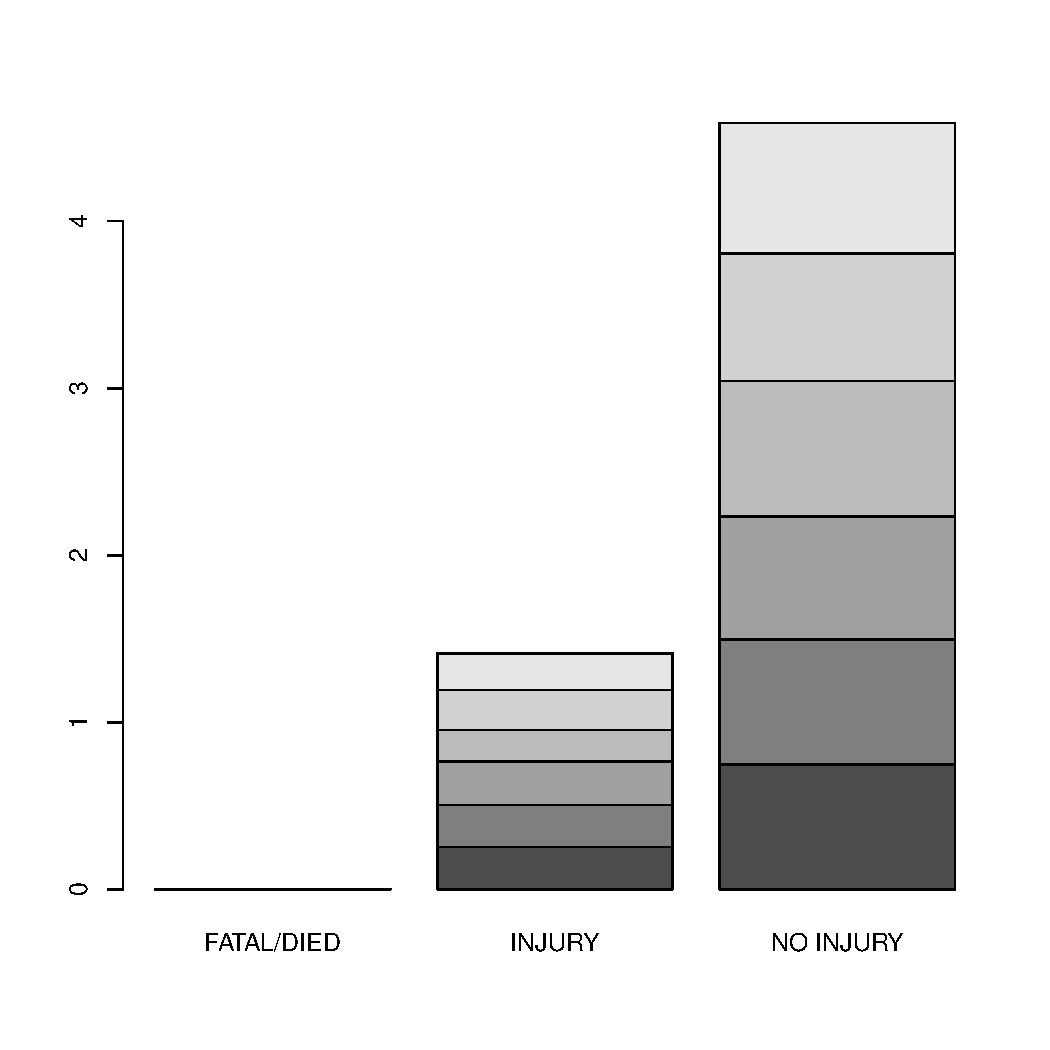
\includegraphics[width=\maxwidth]{figure/unnamed-chunk-9-1} 
\end{knitrout}

We can see that most of the accidents occur during the daytime, with a semi-continuous increasing and decreasing structure. The distribution reaches its lowest value at 3:00AM, and peaks around 4:00PM. There are slight spikes around 8-9AM, when people would be driving to work, and also around 4-5:00PM, when people would be leaving work. There is also a small spike around midnight.

\subsection{Injuries by Person Type}

This series of box plots focuses on collisions that resulted in at least 10 total injuries. We compare the total number of people injured with the amounts of people injured of different types: pedestrians, motorists, and cyclists.

\begin{knitrout}
\definecolor{shadecolor}{rgb}{0.969, 0.969, 0.969}\color{fgcolor}\begin{kframe}
\begin{alltt}
\hldef{people_injured} \hlkwb{<-} \hldef{nyc}\hlopt{$}\hldef{NUMBER.OF.PERSONS.INJURED}
\hldef{pedestrians_injured} \hlkwb{<-} \hldef{nyc}\hlopt{$}\hldef{NUMBER.OF.PEDESTRIANS.INJURED}
\hldef{motorists_injured} \hlkwb{<-} \hldef{nyc}\hlopt{$}\hldef{NUMBER.OF.MOTORIST.INJURED}
\hldef{cyclists_injured} \hlkwb{<-} \hldef{nyc}\hlopt{$}\hldef{NUMBER.OF.CYCLIST.INJURED}

\hldef{mass_factor} \hlkwb{<-} \hldef{people_injured} \hlopt{>=} \hlnum{10}
\hldef{people_injured_mass} \hlkwb{<-} \hldef{people_injured[mass_factor]}
\hldef{motorists_injured_mass} \hlkwb{<-} \hldef{motorists_injured[mass_factor]}
\hldef{pedestrians_injured_mass} \hlkwb{<-} \hldef{pedestrians_injured[mass_factor]}
\hldef{cyclists_injured_mass} \hlkwb{<-} \hldef{cyclists_injured[mass_factor]}
\hlkwd{layout}\hldef{(}\hlkwc{mat} \hldef{=} \hlkwd{matrix}\hldef{(}\hlkwd{c}\hldef{(}\hlnum{1}\hldef{,} \hlnum{2}\hldef{,} \hlnum{3}\hldef{,} \hlnum{4}\hldef{),} \hlnum{4}\hldef{,} \hlkwc{byrow} \hldef{=} \hlnum{TRUE}\hldef{))}
\hlkwd{boxplot}\hldef{(people_injured_mass,}
        \hlkwc{main}\hldef{=}\hlsng{"total people injured for mass casualty events 
        (over 10 people injured)"}\hldef{,}
        \hlkwc{horizontal}\hldef{=}\hlnum{TRUE}\hldef{,} \hlkwc{ylim} \hldef{=} \hlkwd{c}\hldef{(}\hlnum{0}\hldef{,} \hlnum{45}\hldef{))}
\hlkwd{boxplot}\hldef{(motorists_injured_mass,} \hlkwc{main}\hldef{=}\hlsng{"motorists injured"}\hldef{,}
        \hlkwc{horizontal}\hldef{=}\hlnum{TRUE}\hldef{,} \hlkwc{ylim} \hldef{=} \hlkwd{c}\hldef{(}\hlnum{0}\hldef{,} \hlnum{45}\hldef{))}
\hlkwd{boxplot}\hldef{(pedestrians_injured_mass,} \hlkwc{main}\hldef{=}\hlsng{"pedestrians injured"}\hldef{,}
        \hlkwc{horizontal}\hldef{=}\hlnum{TRUE}\hldef{,} \hlkwc{ylim} \hldef{=} \hlkwd{c}\hldef{(}\hlnum{0}\hldef{,} \hlnum{45}\hldef{))}
\hlkwd{boxplot}\hldef{(cyclists_injured_mass,} \hlkwc{main} \hldef{=} \hlsng{"cyclists injured"}\hldef{,}
        \hlkwc{horizontal}\hldef{=}\hlnum{TRUE}\hldef{,} \hlkwc{ylim} \hldef{=} \hlkwd{c}\hldef{(}\hlnum{0}\hldef{,} \hlnum{45}\hldef{))}
\end{alltt}
\end{kframe}
\includegraphics[width=\maxwidth]{figure/unnamed-chunk-10-1} 
\end{knitrout}

The vast majority of these collisions resulted in motorists being the main affected group. This is unsurprising, as every collision must involve motorists, but the other possible parties may not even be present. Pedestrians were mostly uninjured by these collisions, with some exceptions that result in the amount of pedestrian injuries to go into the 20s. Cyclists were the most unaffected by these mass injury collisions, with a couple of collisions injuring one cyclist, but otherwise 0 cyclists were injured in any of the other collisions. 


\subsection{Borough VS Injury Severity}

\subsubsection{Contingency Table}

This contingency table examines whether crash severity (fatal, injury, or no injury) varies across NYC boroughs.

\begin{knitrout}
\definecolor{shadecolor}{rgb}{0.969, 0.969, 0.969}\color{fgcolor}\begin{kframe}
\begin{alltt}
\hldef{nyc}\hlopt{$}\hldef{injury_severity} \hlkwb{<-} \hlkwd{ifelse}\hldef{(nyc}\hlopt{$}\hldef{NUMBER.OF.CYCLIST.KILLED} \hlopt{>} \hlnum{0}\hldef{,}
                              \hlsng{"FATAL/DIED"}\hldef{,}
                       \hlkwd{ifelse}\hldef{(nyc}\hlopt{$}\hldef{NUMBER.OF.PERSONS.INJURED} \hlopt{>} \hlnum{0}\hldef{,}
                              \hlsng{"INJURY"}\hldef{,} \hlsng{"NO INJURY"}\hldef{))}


\hlcom{# removing NA's}
\hldef{borough_injury_data} \hlkwb{<-} \hldef{nyc[}\hlopt{!}\hlkwd{is.na}\hldef{(nyc}\hlopt{$}\hldef{BOROUGH)} \hlopt{& !}\hlkwd{is.na}\hldef{(nyc}\hlopt{$}\hldef{injury_severity), ]}

\hlcom{# Contingency Table}
\hldef{(borough_injury_table} \hlkwb{<-} \hlkwd{table}\hldef{(borough_injury_data}\hlopt{$}\hldef{BOROUGH,}
                               \hldef{borough_injury_data}\hlopt{$}\hldef{injury_severity))}
\end{alltt}
\begin{verbatim}
##                
##                 FATAL/DIED INJURY NO INJURY
##                         75 170997    506210
##   BRONX                 30  57186    169143
##   BROOKLYN              75 127827    361518
##   MANHATTAN             48  64000    274797
##   QUEENS                40  97339    312283
##   STATEN ISLAND          4  14005     50023
\end{verbatim}
\end{kframe}
\end{knitrout}

\begin{knitrout}
\definecolor{shadecolor}{rgb}{0.969, 0.969, 0.969}\color{fgcolor}\begin{kframe}
\begin{alltt}
\hlcom{# Chi-square test}
\hldef{(chi_test1} \hlkwb{<-} \hlkwd{chisq.test}\hldef{(borough_injury_table))}
\end{alltt}
\begin{verbatim}
## 
## 	Pearson's Chi-squared test
## 
## data:  borough_injury_table
## X-squared = 6988.6, df = 10, p-value < 2.2e-16
\end{verbatim}
\end{kframe}
\end{knitrout}

Since p-value < alpha = 0.05, we reject the null hypothesis and conclude that we have sufficient evidence to prove the true population of boroughs are not evenly distributed or in other words, that the distribution of fatal, injury, and property-damage-only crashes varies significantly across NYC boroughs (Chi-square, df=8, p-value < 0.0001). Furthermore, there is a massive test statistic of $X^2$ = 6377.3 which shows the huge differences between what we'd expect if boroughs were all the same vs. what we actually observe.


\subsubsection{Barplot of Row Proportions (by Borough)}
This barplot shows crash severity proportions within each borough.

\begin{knitrout}
\definecolor{shadecolor}{rgb}{0.969, 0.969, 0.969}\color{fgcolor}\begin{kframe}
\begin{alltt}
\hldef{(prop_table1} \hlkwb{<-} \hlkwd{prop.table}\hldef{(borough_injury_table,} \hlkwc{margin} \hldef{=} \hlnum{1}\hldef{))}
\end{alltt}
\begin{verbatim}
##                
##                   FATAL/DIED       INJURY    NO INJURY
##                 1.107367e-04 2.524753e-01 7.474139e-01
##   BRONX         1.325328e-04 2.526341e-01 7.472334e-01
##   BROOKLYN      1.532426e-04 2.611806e-01 7.386662e-01
##   MANHATTAN     1.416577e-04 1.888769e-01 8.109814e-01
##   QUEENS        9.764147e-05 2.376081e-01 7.622943e-01
##   STATEN ISLAND 6.246877e-05 2.187188e-01 7.812188e-01
\end{verbatim}
\begin{alltt}
\hlkwd{barplot}\hldef{(prop_table1)}
\end{alltt}
\end{kframe}
\includegraphics[width=\maxwidth]{figure/unnamed-chunk-13-1} 
\end{knitrout}

While all boroughs have low fatal crash rates (around 0.1-0.16\%), Staten Island has the highest fatality rate at 0.159\%, followed by Brooklyn at 0.142\%. Manhattan appears to be the safest borough with the lowest rates of both fatal (0.107\%) and injury crashes (18.9\%). Brooklyn and the Bronx have the highest injury rates at 26.1\% and 25.3\% respectively, while Manhattan has significantly more no injury crashes (80.1\%) compared to other boroughs.

\subsubsection{Cramer’s V}

\begin{knitrout}
\definecolor{shadecolor}{rgb}{0.969, 0.969, 0.969}\color{fgcolor}\begin{kframe}
\begin{alltt}
\hlkwd{cramerV}\hldef{(borough_injury_table)}
\end{alltt}
\begin{verbatim}
## Cramer V 
##   0.0398
\end{verbatim}
\end{kframe}
\end{knitrout}

The chi-square test concluded that there is a statistically significant association between borough and crash severity. However, the effect size was very small (Cramer's V = 0.046), indicating that while borough differences are statistically detectable, they explain less than 1\% of the variation in crash severity. This suggests that factors other than borough location are much more important in determining crash outcomes.

\subsection{Total Persons Injured vs Killed}

This scatterplot examines the relationship between injuries and fatalities in NYC vehicle crashes.

\begin{knitrout}
\definecolor{shadecolor}{rgb}{0.969, 0.969, 0.969}\color{fgcolor}\begin{kframe}
\begin{alltt}
\hldef{injury_data} \hlkwb{<-} \hldef{nyc[nyc}\hlopt{$}\hldef{NUMBER.OF.PERSONS.INJURED} \hlopt{>} \hlnum{0} \hlopt{|}
                     \hldef{nyc}\hlopt{$}\hldef{NUMBER.OF.PERSONS.KILLED} \hlopt{>} \hlnum{0}\hldef{, ]}

\hlkwd{plot}\hldef{(injury_data}\hlopt{$}\hldef{NUMBER.OF.PERSONS.INJURED,}
     \hldef{injury_data}\hlopt{$}\hldef{NUMBER.OF.PERSONS.KILLED,}
     \hlkwc{main} \hldef{=} \hlsng{"Relationship Between Injuries and Fatalities in NYC Crashes"}\hldef{,}
     \hlkwc{xlab} \hldef{=} \hlsng{"Number of Persons Injured"}\hldef{,}
     \hlkwc{ylab} \hldef{=} \hlsng{"Number of Persons Killed"}\hldef{,}
     \hlkwc{pch} \hldef{=} \hlnum{16}\hldef{,}
     \hlkwc{col} \hldef{=} \hlsng{"darkblue"}\hldef{,}
     \hlkwc{cex} \hldef{=} \hlnum{0.6}\hldef{)}

\hlkwd{abline}\hldef{(}\hlkwd{lm}\hldef{(injury_data}\hlopt{$}\hldef{NUMBER.OF.PERSONS.KILLED} \hlopt{~}
            \hldef{injury_data}\hlopt{$}\hldef{NUMBER.OF.PERSONS.INJURED),}
       \hlkwc{col} \hldef{=} \hlsng{"red"}\hldef{,} \hlkwc{lwd} \hldef{=} \hlnum{2}\hldef{)}
\end{alltt}
\end{kframe}
\includegraphics[width=\maxwidth]{figure/unnamed-chunk-15-1} 
\end{knitrout}

The plot shows that most crashes result in injuries but no deaths which can be seen by the concentration of points along the bottom. Fatal crashes are rare and scattered across injury levels, with no clear correlation. The flat regression line shows that there is a minimal relationship between injuries and deaths, suggesting fatalities depend more on crash circumstances than the number of people involved.


\subsection{Density of Injuries per Borough}

This jitter plot is showing the distribution of the number of people injured per incident across different boroughs, while avoiding overplotting so patterns in the data density can be seen.

\begin{knitrout}
\definecolor{shadecolor}{rgb}{0.969, 0.969, 0.969}\color{fgcolor}\begin{kframe}
\begin{alltt}
\hlkwd{ggplot}\hldef{(nyc} \hlopt \hlkwd{filter}\hldef{(BOROUGH} \hlopt{!=} \hlsng{""}\hldef{))} \hlopt{+}
  \hlkwd{aes}\hldef{(}\hlkwc{x}\hldef{=BOROUGH,} \hlkwc{y}\hldef{=NUMBER.OF.PERSONS.INJURED)} \hlopt{+}
  \hlkwd{coord_cartesian}\hldef{(}\hlkwc{ylim} \hldef{=} \hlkwd{c}\hldef{(}\hlnum{0}\hldef{,} \hlnum{10}\hldef{))} \hlopt{+}
  \hlkwd{scale_y_continuous}\hldef{(}\hlkwc{breaks} \hldef{=} \hlkwd{seq}\hldef{(}\hlnum{0}\hldef{,} \hlnum{10}\hldef{,} \hlnum{1}\hldef{))} \hlopt{+}
  \hlkwd{labs}\hldef{(}
    \hlkwc{x} \hldef{=} \hlsng{"Borough"}\hldef{,}
    \hlkwc{y} \hldef{=} \hlsng{"Number of Persons Injured"}\hldef{,}
    \hlkwc{title} \hldef{=} \hlsng{"Density of Injuries per Borough"}
    \hldef{)} \hlopt{+}
  \hlkwd{geom_jitter}\hldef{(}\hlkwc{alpha} \hldef{=} \hlnum{1}\hlopt{/}\hlnum{25}\hldef{)}
\end{alltt}


{\ttfamily\noindent\color{warningcolor}{\#\# Warning: Removed 11 rows containing missing values or values outside the scale range\\\#\# (`geom\_point()`).}}\end{kframe}
\includegraphics[width=\maxwidth]{figure/unnamed-chunk-16-1} 
\end{knitrout}

This jitter plot shows the distribution of the number of persons injured per crash across NYC boroughs. Most crashes result in 0–3 injuries (dark dense bands at the bottom). Brooklyn and Queens display more incidents with higher injury counts, indicating that crashes in these boroughs tend to involve more people. Manhattan, despite its high traffic, has relatively fewer multi-injury crashes compared to Brooklyn or the Bronx. Staten Island stands out with the least severe crashes (it is the least populated and least densely built borough), with most incidents involving very few or no injuries.


\subsection{Crash Frequency by Hour and Day of Week}

To explore when crashes are most likely to occur, we created a heatmap of crash counts by hour of the day and day of the week. Each tile represents the total number of crashes in that time slot, with brighter colors indicating more frequent crashes.

\begin{knitrout}
\definecolor{shadecolor}{rgb}{0.969, 0.969, 0.969}\color{fgcolor}\begin{kframe}
\begin{alltt}
\hldef{nyc} \hlopt
  \hlkwd{mutate}\hldef{(}
    \hlkwc{hour} \hldef{=} \hlkwd{hour}\hldef{(}\hlkwd{hm}\hldef{(CRASH.TIME)),}
    \hlkwc{date} \hldef{=} \hlkwd{ymd}\hldef{(CRASH.DATE),}
    \hlkwc{weekday} \hldef{=} \hlkwd{wday}\hldef{(date,} \hlkwc{label} \hldef{=} \hlnum{TRUE}\hldef{,} \hlkwc{abbr} \hldef{=} \hlnum{FALSE}\hldef{)}
  \hldef{)} \hlopt
  \hlkwd{count}\hldef{(hour, weekday)} \hlopt
  \hlkwd{ggplot}\hldef{(}\hlkwd{aes}\hldef{(}\hlkwc{x} \hldef{= hour,} \hlkwc{y} \hldef{= weekday,} \hlkwc{fill} \hldef{= n))} \hlopt{+}
  \hlkwd{geom_tile}\hldef{(}\hlkwc{color} \hldef{=} \hlsng{"white"}\hldef{)} \hlopt{+}
  \hlkwd{scale_fill_viridis_c}\hldef{(}\hlkwc{option} \hldef{=} \hlsng{"C"}\hldef{)} \hlopt{+}
  \hlkwd{labs}\hldef{(}
    \hlkwc{title} \hldef{=} \hlsng{"Crash Frequency by Hour and Day of Week"}\hldef{,}
    \hlkwc{x} \hldef{=} \hlsng{"Hour of Day"}\hldef{,}
    \hlkwc{y} \hldef{=} \hlsng{"Day of Week"}\hldef{,}
    \hlkwc{fill} \hldef{=} \hlsng{"Number of Crashes"}
  \hldef{)} \hlopt{+}
  \hlkwd{theme_minimal}\hldef{()}
\end{alltt}
\end{kframe}
\includegraphics[width=\maxwidth]{figure/unnamed-chunk-17-1} 
\end{knitrout}

The heatmap shows a clear concentration of crashes during daytime and evening hours, especially between 8 AM and 7 PM across all weekdays. Friday stands out with the highest crash intensity, particularly in the late afternoon and early evening, likely reflecting a mix of rush-hour traffic and increased social activity at the end of the work week.

In contrast, the overnight hours (midnight to 6 AM) consistently display the fewest crashes across all days, reflecting lower traffic volumes during those times. Sundays appear somewhat less intense overall compared to weekdays, with a broader distribution of crashes throughout the afternoon.

Overall, the heatmap highlights how crash risk peaks during high-traffic commuting periods and social activity times, with Friday evenings being particularly hazardous in New York City.

\subsection{Distribution of Vehicle Age Involved in Accidents}
We explore the distribution of vehicle ages involved in collisions across each five boroughs. This data is extracted from one of the secondary datasets, linking the collision ID from the original dataset to the individual vehicles involved in each collision. The resulting histogram is plotted below.

\begin{knitrout}
\definecolor{shadecolor}{rgb}{0.969, 0.969, 0.969}\color{fgcolor}\begin{kframe}
\begin{alltt}
\hlkwd{ggplot}\hldef{(}\hlkwc{data}\hldef{=nyc[}\hlopt{!}\hlkwd{is.na}\hldef{(nyc}\hlopt{$}\hldef{AV_VEH_AGE)} \hlopt{&} \hldef{nyc}\hlopt{$}\hldef{BOROUGH} \hlopt{!=}\hlsng{""}\hldef{, ])} \hlopt{+}
    \hlkwd{aes}\hldef{(AV_VEH_AGE, ..density..,} \hlkwc{fill} \hldef{= BOROUGH)} \hlopt{+}
    \hlkwd{facet_grid}\hldef{(.}\hlopt{~}\hldef{BOROUGH)} \hlopt{+}
    \hlkwd{geom_histogram}\hldef{(}\hlkwc{color} \hldef{=} \hlsng{"black"}\hldef{,} \hlkwc{alpha} \hldef{=} \hlnum{0.7}\hldef{)} \hlopt{+}
    \hlkwd{xlim}\hldef{(}\hlkwd{c}\hldef{(}\hlnum{0}\hldef{,}\hlnum{30}\hldef{))} \hlopt{+}
    \hlkwd{labs}\hldef{(}\hlkwc{title} \hldef{=} \hlsng{"Distribution of Vehicle Age by Borough"}\hldef{,}
         \hlkwc{x} \hldef{=} \hlsng{"Average Vehicle Age (Years)"}\hldef{,}
         \hlkwc{y} \hldef{=} \hlsng{"Density"}\hldef{)} \hlopt{+}
    \hlkwd{theme}\hldef{(}\hlkwc{legend.position} \hldef{=} \hlsng{"none"}\hldef{)}
\end{alltt}


{\ttfamily\noindent\color{warningcolor}{\#\# Warning: The dot-dot notation (`..density..`) was deprecated in ggplot2 3.4.0.\\\#\# i Please use `after\_stat(density)` instead.\\\#\# This warning is displayed once every 8 hours.\\\#\# Call `lifecycle::last\_lifecycle\_warnings()` to see where this warning was\\\#\# generated.}}

{\ttfamily\noindent\itshape\color{messagecolor}{\#\# `stat\_bin()` using `bins = 30`. Pick better value `binwidth`.}}

{\ttfamily\noindent\color{warningcolor}{\#\# Warning: Removed 575 rows containing non-finite outside the scale range (`stat\_bin()`).}}

{\ttfamily\noindent\color{warningcolor}{\#\# Warning: Removed 10 rows containing missing values or values outside the scale range\\\#\# (`geom\_bar()`).}}\end{kframe}
\includegraphics[width=\maxwidth]{figure/unnamed-chunk-18-1} 
\end{knitrout}
The distributions appear similar for each borough, with the notable exception of Manhattan, which appears to have a generally younger age of cars among collisions. This can be mostly attributed to the greater wealth found in Manhattan. To see real trends between car age and collisions the next step will be to compare against the overall frequency of cars on the road.

\subsection{Accidents and speed limits on NYC map}

\subsubsection{All Accidents}

There are two graphs plotted below. One superimposes a subset of the accidents on the map of NYC, color coded by borough, and the other superimposes a subset of the speed limits on the map of NYC. 

\begin{knitrout}
\definecolor{shadecolor}{rgb}{0.969, 0.969, 0.969}\color{fgcolor}\begin{kframe}
\begin{alltt}
\hlcom{#plot the car crashes on the NYC map}
\hldef{has_long_lat} \hlkwb{<-} \hldef{nyc[}\hlopt{!}\hlkwd{is.na}\hldef{(nyc}\hlopt{$}\hldef{LONGITUDE)} \hlopt{& !}\hlkwd{is.na}\hldef{(nyc}\hlopt{$}\hldef{LATITUDE),]}
\hldef{no_outliers} \hlkwb{<-} \hldef{has_long_lat[}
  \hldef{has_long_lat}\hlopt{$}\hldef{LONGITUDE} \hlopt{> -}\hlnum{74.26} \hlopt{&}
    \hldef{has_long_lat}\hlopt{$}\hldef{LONGITUDE} \hlopt{< -}\hlnum{73.70} \hlopt{&}
    \hldef{has_long_lat}\hlopt{$}\hldef{LATITUDE} \hlopt{>} \hlnum{40.49} \hlopt{&}
    \hldef{has_long_lat}\hlopt{$}\hldef{LATITUDE} \hlopt{<} \hlnum{40.92}\hldef{, ]}

\hldef{small_sample} \hlkwb{<-} \hldef{no_outliers[}\hlkwd{sample}\hldef{(}\hlkwd{nrow}\hldef{(no_outliers),} \hlnum{3000}\hldef{),]}
\hldef{boroughs} \hlkwb{<-} \hldef{small_sample}\hlopt{$}\hldef{BOROUGH}
\hldef{small_sample_sf} \hlkwb{<-} \hlkwd{st_as_sf}\hldef{(small_sample,} \hlkwc{coords} \hldef{=} \hlkwd{c}\hldef{(}\hlsng{"LONGITUDE"}\hldef{,} \hlsng{"LATITUDE"}\hldef{),} \hlkwc{crs} \hldef{=} \hlnum{4326}\hldef{)}
\hldef{small_sample_sf} \hlkwb{<-} \hlkwd{st_transform}\hldef{(small_sample_sf,} \hlnum{3857}\hldef{)}
\hldef{nyc_bbox} \hlkwb{<-} \hlkwd{st_bbox}\hldef{(small_sample_sf)}

\hldef{accident_plot} \hlkwb{<-} \hlkwd{ggplot}\hldef{()} \hlopt{+}
  \hlkwd{annotation_map_tile}\hldef{(}\hlkwc{type} \hldef{=} \hlsng{"cartolight"}\hldef{,} \hlkwc{zoom} \hldef{=} \hlnum{11}\hldef{)} \hlopt{+}
  \hlkwd{aes}\hldef{(}\hlkwc{color} \hldef{= boroughs)} \hlopt{+}
  \hlkwd{geom_sf}\hldef{(}\hlkwc{data} \hldef{= small_sample_sf,} \hlkwc{size} \hldef{=} \hlnum{1}\hldef{)} \hlopt{+}
  \hlkwd{coord_sf}\hldef{(}\hlkwc{xlim} \hldef{=} \hlkwd{c}\hldef{(nyc_bbox[}\hlsng{"xmin"}\hldef{], nyc_bbox[}\hlsng{"xmax"}\hldef{]),}
           \hlkwc{ylim} \hldef{=} \hlkwd{c}\hldef{(nyc_bbox[}\hlsng{"ymin"}\hldef{], nyc_bbox[}\hlsng{"ymax"}\hldef{]),}
           \hlkwc{expand} \hldef{=} \hlnum{FALSE}\hldef{)} \hlopt{+}
  \hlkwd{labs}\hldef{(}\hlkwc{title} \hldef{=} \hlsng{"NYC Accident Mapping by Borough"}\hldef{)}


\hlcom{# plot the speed limits on the NYC map}
\hldef{no_outliers_sp} \hlkwb{<-} \hldef{sp_limits[}
  \hldef{sp_limits}\hlopt{$}\hldef{longitude} \hlopt{> -}\hlnum{74.26} \hlopt{&}
    \hldef{sp_limits}\hlopt{$}\hldef{longitude} \hlopt{< -}\hlnum{73.70} \hlopt{&}
    \hldef{sp_limits}\hlopt{$}\hldef{latitude} \hlopt{>} \hlnum{40.49} \hlopt{&}
    \hldef{sp_limits}\hlopt{$}\hldef{latitude} \hlopt{<} \hlnum{40.92}\hldef{, ]}
\hldef{small_sp_sample} \hlkwb{<-} \hldef{no_outliers_sp[}\hlkwd{sample}\hldef{(}\hlkwd{nrow}\hldef{(no_outliers_sp),} \hlnum{8000}\hldef{),]}
\hldef{speeds} \hlkwb{<-} \hldef{small_sp_sample}\hlopt{$}\hldef{postvz_sl}
\hldef{small_sp_sample_sf} \hlkwb{<-} \hlkwd{st_as_sf}\hldef{(small_sp_sample,} \hlkwc{coords} \hldef{=} \hlkwd{c}\hldef{(}\hlsng{"longitude"}\hldef{,} \hlsng{"latitude"}\hldef{),} \hlkwc{crs} \hldef{=} \hlnum{4326}\hldef{)}
\hldef{small_sp_sample_sf} \hlkwb{<-} \hlkwd{st_transform}\hldef{(small_sp_sample_sf,} \hlnum{3857}\hldef{)}
\hldef{speed_plot} \hlkwb{<-} \hlkwd{ggplot}\hldef{()}\hlopt{+}
  \hlkwd{annotation_map_tile}\hldef{(}\hlkwc{type} \hldef{=} \hlsng{"cartolight"}\hldef{,} \hlkwc{zoom} \hldef{=} \hlnum{11}\hldef{)} \hlopt{+}
  \hlkwd{aes}\hldef{(}\hlkwc{color} \hldef{= speeds)} \hlopt{+}
  \hlkwd{geom_sf}\hldef{(}\hlkwc{data} \hldef{= small_sp_sample_sf,} \hlkwc{size} \hldef{=} \hlnum{1}\hldef{)} \hlopt{+}
  \hlkwd{coord_sf}\hldef{(}\hlkwc{xlim} \hldef{=} \hlkwd{c}\hldef{(nyc_bbox[}\hlsng{"xmin"}\hldef{], nyc_bbox[}\hlsng{"xmax"}\hldef{]),}
           \hlkwc{ylim} \hldef{=} \hlkwd{c}\hldef{(nyc_bbox[}\hlsng{"ymin"}\hldef{], nyc_bbox[}\hlsng{"ymax"}\hldef{]),}
           \hlkwc{expand} \hldef{=} \hlnum{FALSE}\hldef{)} \hlopt{+}
  \hlkwd{labs}\hldef{(}\hlkwc{title} \hldef{=} \hlsng{"NYC Speed Limit Mapping"}\hldef{)} \hlopt{+}
  \hlkwd{scale_color_gradient}\hldef{(}\hlkwc{low} \hldef{=} \hlsng{"green"}\hldef{,} \hlkwc{high} \hldef{=} \hlsng{"red"}\hldef{)}


\hlcom{# Display plots side by side}
\hlkwd{require}\hldef{(gridExtra)}
\hlkwd{grid.arrange}\hldef{(accident_plot,speed_plot)}
\end{alltt}


{\ttfamily\noindent\itshape\color{messagecolor}{\#\# Zoom: 11\\\#\# Zoom: 11}}\end{kframe}
\includegraphics[width=\maxwidth]{figure/unnamed-chunk-19-1} 
\end{knitrout}

The speed limit graph shows that there are high speed limits on the highways, around the 40-50mph range, and lower speed limits everywhere else, mostly in the 20-30mph range. We can visually inspect and see that a lot of the areas that did not have labels for their borough correspond with the higher speed limit lines, indicating that when an accident occurred on a highway, there was likely no borough provided. We can also see that a lot of the accidents are focused in the Manhattan area, with the most sparse area being Staten Island. This is likely because of the street density in Manhattan vs Staten Island.

\subsubsection{Highway Accidents}

Below, we have a graph showing all of the accidents that occurred on roads where the speed limit is greater than 40 mph, mapped onto an image of NYC. This gives us a far clearer picture of the highway road mapping in NYC.

\begin{knitrout}
\definecolor{shadecolor}{rgb}{0.969, 0.969, 0.969}\color{fgcolor}\begin{kframe}
\begin{alltt}
\hlcom{# Find the accidents that occurred on high speed roads}
\hldef{highways} \hlkwb{<-} \hldef{sp_limits[sp_limits}\hlopt{$}\hldef{postvz_sl} \hlopt{>} \hlnum{40}\hldef{, ]}
\hldef{nyc}\hlopt{$}\hldef{HIGHWAY} \hlkwb{<-} \hldef{nyc}\hlopt{$}\hldef{round_location} \hlopt \hldef{highways}\hlopt{$}\hldef{location}
\hldef{hwy_accidents} \hlkwb{<-} \hldef{nyc[nyc}\hlopt{$}\hldef{HIGHWAY} \hlopt{==} \hlnum{TRUE}\hldef{, ]}
\hldef{hwy_accidents_sf} \hlkwb{<-} \hlkwd{st_as_sf}\hldef{(hwy_accidents,} \hlkwc{coords} \hldef{=} \hlkwd{c}\hldef{(}\hlsng{"LONGITUDE"}\hldef{,} \hlsng{"LATITUDE"}\hldef{),} \hlkwc{crs} \hldef{=} \hlnum{4326}\hldef{)}
\hldef{hwy_accidents_sf} \hlkwb{<-} \hlkwd{st_transform}\hldef{(hwy_accidents_sf,} \hlnum{3857}\hldef{)}
\hldef{nyc_bbox} \hlkwb{<-} \hlkwd{st_bbox}\hldef{(hwy_accidents_sf)}

\hlkwd{ggplot}\hldef{()} \hlopt{+}
  \hlkwd{annotation_map_tile}\hldef{(}\hlkwc{type} \hldef{=} \hlsng{"cartolight"}\hldef{,} \hlkwc{zoom} \hldef{=} \hlnum{11}\hldef{)} \hlopt{+}
  \hlkwd{geom_sf}\hldef{(}\hlkwc{data} \hldef{= hwy_accidents_sf,} \hlkwc{size} \hldef{=} \hlnum{1}\hldef{)} \hlopt{+}
  \hlkwd{coord_sf}\hldef{(}\hlkwc{xlim} \hldef{=} \hlkwd{c}\hldef{(nyc_bbox[}\hlsng{"xmin"}\hldef{], nyc_bbox[}\hlsng{"xmax"}\hldef{]),}
           \hlkwc{ylim} \hldef{=} \hlkwd{c}\hldef{(nyc_bbox[}\hlsng{"ymin"}\hldef{], nyc_bbox[}\hlsng{"ymax"}\hldef{]),}
           \hlkwc{expand} \hldef{=} \hlnum{FALSE}\hldef{)} \hlopt{+}
  \hlkwd{labs}\hldef{(}\hlkwc{title} \hldef{=} \hlsng{"Car accidents on high speed roads (>40mph)"}\hldef{)}
\end{alltt}


{\ttfamily\noindent\itshape\color{messagecolor}{\#\# Zoom: 11}}\end{kframe}
\includegraphics[width=\maxwidth]{figure/unnamed-chunk-20-1} 
\end{knitrout}

While this imaging doesn’t directly allow us to draw any conclusions, having this mapping of which car accidents occurred on higher speed roads allows us to do further interpretations of the data with relation to the speed limit, as we show in the next graphical comparison. 


\subsection{Density Comparison of Times of Day for Car Accidents: Highway Vs Not Highway}

Here we combine our supplementary dataset with our main dataset to compare the car accidents that have occurred on higher speed roads vs those that have occurred on lower speed roads. The density plot is shown below.

\begin{knitrout}
\definecolor{shadecolor}{rgb}{0.969, 0.969, 0.969}\color{fgcolor}\begin{kframe}
\begin{alltt}
\hlcom{# plot the hours vs the hours}

\hldef{hwy_accidents} \hlkwb{<-} \hldef{nyc[nyc}\hlopt{$}\hldef{HIGHWAY} \hlopt{==} \hlnum{TRUE}\hldef{, ]}
\hldef{nyc_sample} \hlkwb{<-} \hldef{nyc[}\hlkwd{sample}\hldef{(}\hlkwd{nrow}\hldef{(nyc),} \hlkwd{nrow}\hldef{(hwy_accidents)),]}

\hldef{combined} \hlkwb{<-} \hlkwd{rbind}\hldef{(nyc_sample, hwy_accidents)}
\hlkwd{ggplot}\hldef{(combined,} \hlkwd{aes}\hldef{(}\hlkwc{x} \hldef{= HOUR,} \hlkwc{fill} \hldef{= HIGHWAY))} \hlopt{+}
  \hlkwd{geom_density}\hldef{(}\hlkwc{position} \hldef{=} \hlsng{"identity"}\hldef{,} \hlkwc{alpha} \hldef{=} \hlnum{0.5}\hldef{)} \hlopt{+}
  \hlkwd{scale_x_discrete}\hldef{(}\hlkwc{labels}\hldef{=}\hlkwd{c}\hldef{(}\hlsng{"custom"}\hldef{,} \hlsng{"label"}\hldef{))} \hlopt{+}
  \hlkwd{scale_x_continuous}\hldef{(}\hlkwc{breaks} \hldef{=} \hlkwd{c}\hldef{(}\hlnum{0}\hldef{,} \hlnum{3}\hldef{,} \hlnum{6}\hldef{,} \hlnum{9}\hldef{,} \hlnum{12}\hldef{,} \hlnum{15}\hldef{,} \hlnum{18}\hldef{,} \hlnum{21}\hldef{),} \hlkwc{labels} \hldef{=} \hlkwd{c}\hldef{(}\hlsng{"Midnight"}\hldef{,} \hlsng{"3:00AM"}\hldef{,} \hlsng{"6:00AM"}\hldef{,}\hlsng{"9:00AM"}\hldef{,} \hlsng{"Noon"}\hldef{,} \hlsng{"3:00PM"}\hldef{,} \hlsng{"6:00PM"}\hldef{,} \hlsng{"9:00PM"}\hldef{))}\hlopt{+}
  \hlkwd{scale_fill_discrete}\hldef{(}\hlkwc{labels} \hldef{=} \hlkwd{c}\hldef{(}\hlsng{'Low speed road (<40 mph)'}\hldef{,} \hlsng{'High speed road (>40 mph)'}\hldef{))} \hlopt{+}
  \hlkwd{xlab}\hldef{(}\hlsng{"time of day"}\hldef{)} \hlopt{+} \hlkwd{ggtitle}\hldef{(}\hlsng{"comparison of densities of times of car accidents on highways vs streets"}\hldef{)}
\end{alltt}


{\ttfamily\noindent\itshape\color{messagecolor}{\#\# Scale for x is already present.\\\#\# Adding another scale for x, which will replace the existing scale.}}\end{kframe}
\includegraphics[width=\maxwidth]{figure/unnamed-chunk-21-1} 
\end{knitrout}

We can see from this density plot that the accidents that have occurred on highways have more significant peaks at around 8:00AM and 4:00PM, during people’s work commutes in and out of the city. The accidents that have occurred on regular roads are less predictable, with more occurrences in the middle of the day during traditional working hours.


\section{Preliminary Statistical Modeling \& Interpretation}

To better understand the factors that influence the severity of motor vehicle collisions in New York City, we developed a preliminary statistical model using logistic regression. The outcome of interest is whether a crash was fatal (at least one person killed) or non-fatal. Logistic regression is appropriate in this context because the outcome is binary (fatal vs. non-fatal), and it allows us to estimate how different factors change the odds of a fatal crash while holding other conditions constant.

In simple terms, the model compares patterns across thousands of crashes to estimate how likely a fatal outcome is under different conditions. For example, whether the crash happened at night or involved a motorcycle. The predictors we included were the borough of occurrence, time of day (day vs. night), vehicle type, and the primary contributing factor reported by police. By examining these, we can identify which circumstances or behaviors are most strongly associated with fatal outcomes.

\subsection{Code and Results}


Data cleansing and transformations:
\begin{knitrout}
\definecolor{shadecolor}{rgb}{0.969, 0.969, 0.969}\color{fgcolor}\begin{kframe}
\begin{alltt}
\hldef{nyc_small} \hlkwb{<-} \hldef{nyc} \hlopt
  \hlkwd{filter}\hldef{(BOROUGH} \hlopt{!=} \hlsng{""} \hlopt{&}
           \hldef{CONTRIBUTING.FACTOR.VEHICLE.1} \hlopt{!=} \hlsng{""} \hlopt{&}
           \hldef{CONTRIBUTING.FACTOR.VEHICLE.1} \hlopt{!=} \hlsng{"1"} \hlopt{&}
           \hldef{CONTRIBUTING.FACTOR.VEHICLE.1} \hlopt{!=} \hlsng{"80"}\hldef{)} \hlopt
  \hlkwd{transmute}\hldef{(}
    \hlkwc{is_fatal} \hldef{=} \hlkwd{ifelse}\hldef{(NUMBER.OF.PERSONS.KILLED} \hlopt{>} \hlnum{0}\hldef{,} \hlnum{1}\hldef{,} \hlnum{0}\hldef{),}  \hlcom{# outcome}
    \hlkwc{borough} \hldef{= BOROUGH,}
    \hlkwc{crash_hour} \hldef{=} \hlkwd{hour}\hldef{(}\hlkwd{hm}\hldef{(CRASH.TIME)),}
    \hlkwc{contributing_factor} \hldef{= CONTRIBUTING.FACTOR.VEHICLE.1,}
    \hlkwc{vehicle_cat} \hldef{=} \hlkwd{factor}\hldef{(}\hlkwd{case_when}\hldef{(}
      \hlkwd{grepl}\hldef{(}\hlsng{"MOTORCYCLE|MOTORBIKE"}\hldef{, VEHICLE.TYPE.CODE.1,} \hlkwc{ignore.case} \hldef{=} \hlnum{TRUE}\hldef{)} \hlopt{~}
        \hlsng{"motorcycle"}\hldef{,}
      \hlkwd{grepl}\hldef{(}\hlsng{"TRUCK|BUS"}\hldef{, VEHICLE.TYPE.CODE.1,} \hlkwc{ignore.case} \hldef{=} \hlnum{TRUE}\hldef{)} \hlopt{~}
        \hlsng{"truck_bus"}\hldef{,}
      \hlkwd{grepl}\hldef{(}\hlsng{"BICYCLE|BIKE|SCOOTER"}\hldef{, VEHICLE.TYPE.CODE.1,} \hlkwc{ignore.case} \hldef{=} \hlnum{TRUE}\hldef{)} \hlopt{~}
        \hlsng{"bike_scooter"}\hldef{,}
      \hlnum{TRUE} \hlopt{~} \hlsng{"car_suv"}
    \hldef{))}
  \hldef{)}

\hldef{nyc_small} \hlkwb{<-} \hldef{nyc_small} \hlopt
  \hlkwd{mutate}\hldef{(}\hlkwc{hour} \hldef{=} \hlkwd{as.numeric}\hldef{(}\hlkwd{substr}\hldef{(crash_hour,} \hlnum{1}\hldef{,} \hlnum{2}\hldef{)),}
         \hlkwc{tod} \hldef{=} \hlkwd{ifelse}\hldef{(hour} \hlopt{>=} \hlnum{6} \hlopt{&} \hldef{hour} \hlopt{<} \hlnum{18}\hldef{,} \hlsng{"day"}\hldef{,} \hlsng{"night"}\hldef{))}

\hldef{nyc_small}\hlopt{$}\hldef{BOROUGH} \hlkwb{<-} \hlkwd{droplevels}\hldef{(}\hlkwd{as.factor}\hldef{(nyc_small}\hlopt{$}\hldef{borough))}

\hlcom{# set baselines for model}
\hldef{nyc_small}\hlopt{$}\hldef{borough} \hlkwb{<-} \hlkwd{relevel}\hldef{(}\hlkwd{as.factor}\hldef{(nyc_small}\hlopt{$}\hldef{BOROUGH),}
                             \hlkwc{ref} \hldef{=} \hlsng{"STATEN ISLAND"}\hldef{)}
\hldef{nyc_small}\hlopt{$}\hldef{tod} \hlkwb{<-} \hlkwd{relevel}\hldef{(}\hlkwd{as.factor}\hldef{(nyc_small}\hlopt{$}\hldef{tod),}
                         \hlkwc{ref} \hldef{=} \hlsng{"day"}\hldef{)}
\hldef{nyc_small}\hlopt{$}\hldef{vehicle_cat} \hlkwb{<-} \hlkwd{relevel}\hldef{(}\hlkwd{as.factor}\hldef{(nyc_small}\hlopt{$}\hldef{vehicle_cat),}
                                 \hlkwc{ref} \hldef{=} \hlsng{"car_suv"}\hldef{)}
\hldef{nyc_small}\hlopt{$}\hldef{contributing_factor} \hlkwb{<-} \hlkwd{relevel}\hldef{(}
  \hlkwd{as.factor}\hldef{(nyc_small}\hlopt{$}\hldef{contributing_factor),}\hlkwc{ref} \hldef{=} \hlsng{"Unspecified"}\hldef{)}
\end{alltt}
\end{kframe}
\end{knitrout}

Creating the logistic regression model:
\begin{knitrout}
\definecolor{shadecolor}{rgb}{0.969, 0.969, 0.969}\color{fgcolor}\begin{kframe}
\begin{alltt}
\hldef{model} \hlkwb{<-} \hlkwd{glm}\hldef{(is_fatal} \hlopt{~} \hldef{borough} \hlopt{+} \hldef{tod} \hlopt{+} \hldef{vehicle_cat} \hlopt{+} \hldef{contributing_factor,}
             \hlkwc{data} \hldef{= nyc_small,}
             \hlkwc{family} \hldef{= binomial)}


\hldef{summ} \hlkwb{<-} \hlkwd{summary}\hldef{(model)}

\hldef{coefs} \hlkwb{<-} \hldef{summ}\hlopt{$}\hldef{coefficients}
\hldef{est} \hlkwb{<-} \hldef{coefs[,} \hlsng{"Estimate"}\hldef{]}         \hlcom{# log-odds}
\hldef{se}  \hlkwb{<-} \hldef{coefs[,} \hlsng{"Std. Error"}\hldef{]}       \hlcom{# standard errors}

\hlcom{# compute odds ratios + 95% confidence intervals}
\hldef{ci_low}  \hlkwb{<-} \hlkwd{exp}\hldef{(est} \hlopt{-} \hlnum{1.96} \hlopt{*} \hldef{se)}
\hldef{ci_high} \hlkwb{<-} \hlkwd{exp}\hldef{(est} \hlopt{+} \hlnum{1.96} \hlopt{*} \hldef{se)}

\hldef{results_table} \hlkwb{<-} \hlkwd{data.frame}\hldef{(}
  \hlkwc{term}        \hldef{=} \hlkwd{rownames}\hldef{(coefs),}
  \hlkwc{odds_ratio}  \hldef{=} \hlkwd{exp}\hldef{(est),}
  \hlkwc{ci_low}      \hldef{= ci_low,}
  \hlkwc{ci_high}     \hldef{= ci_high,}
  \hlkwc{significant} \hldef{=} \hlkwd{ifelse}\hldef{(coefs[,} \hlsng{"Pr(>|z|)"}\hldef{]} \hlopt{<} \hlnum{0.05}\hldef{,} \hlsng{"yes"}\hldef{,} \hlsng{"no"}\hldef{),}
  \hlkwc{row.names}   \hldef{=} \hlkwa{NULL}
\hldef{)}

\hlcom{# filter out the intercept/baseline to keep table cleaner}
\hldef{results_table} \hlkwb{<-} \hldef{results_table[results_table}\hlopt{$}\hldef{term} \hlopt{!=} \hlsng{"(Intercept)"}\hldef{, ]}

\hldef{results_table}\hlopt{$}\hldef{term} \hlkwb{<-} \hlkwd{gsub}\hldef{(}\hlsng{"vehicle_cat"}\hldef{,} \hlsng{"Vehicle: "}\hldef{,}
                           \hldef{results_table}\hlopt{$}\hldef{term)}
\hldef{results_table}\hlopt{$}\hldef{term} \hlkwb{<-} \hlkwd{gsub}\hldef{(}\hlsng{"borough"}\hldef{,} \hlsng{"Borough: "}\hldef{,}
                           \hldef{results_table}\hlopt{$}\hldef{term)}
\hldef{results_table}\hlopt{$}\hldef{term} \hlkwb{<-} \hlkwd{gsub}\hldef{(}\hlsng{"tod"}\hldef{,} \hlsng{"Time of Day: "}\hldef{,}
                           \hldef{results_table}\hlopt{$}\hldef{term)}
\hldef{results_table}\hlopt{$}\hldef{term} \hlkwb{<-} \hlkwd{gsub}\hldef{(}\hlsng{"contributing_factor"}\hldef{,} \hlsng{"Contributing Factor: "}\hldef{,}
                           \hldef{results_table}\hlopt{$}\hldef{term)}

\hldef{results_table}
\end{alltt}
\begin{verbatim}
##                                                                          term
## 2                                                              Borough: BRONX
## 3                                                           Borough: BROOKLYN
## 4                                                          Borough: MANHATTAN
## 5                                                             Borough: QUEENS
## 6                                                          Time of Day: night
## 7                                                       Vehicle: bike_scooter
## 8                                                         Vehicle: motorcycle
## 9                                                          Vehicle: truck_bus
## 10                                 Contributing Factor: Accelerator Defective
## 11                          Contributing Factor: Aggressive Driving/Road Rage
## 12                                   Contributing Factor: Alcohol Involvement
## 13                                        Contributing Factor: Animals Action
## 14                                      Contributing Factor: Backing Unsafely
## 15                                      Contributing Factor: Brakes Defective
## 16                                Contributing Factor: Cell Phone (hand-held)
## 17                                Contributing Factor: Cell Phone (hand-Held)
## 18                               Contributing Factor: Cell Phone (hands-free)
## 19                        Contributing Factor: Driver Inattention/Distraction
## 20                                   Contributing Factor: Driver Inexperience
## 21                            Contributing Factor: Driverless/Runaway Vehicle
## 22                                       Contributing Factor: Drugs (illegal)
## 23                                       Contributing Factor: Drugs (Illegal)
## 24                                    Contributing Factor: Eating or Drinking
## 25                                 Contributing Factor: Failure to Keep Right
## 26                         Contributing Factor: Failure to Yield Right-of-Way
## 27                                       Contributing Factor: Fatigued/Drowsy
## 28                                           Contributing Factor: Fell Asleep
## 29                                 Contributing Factor: Following Too Closely
## 30                                                 Contributing Factor: Glare
## 31                                  Contributing Factor: Headlights Defective
## 32                                                Contributing Factor: Illnes
## 33                                               Contributing Factor: Illness
## 34                      Contributing Factor: Lane Marking Improper/Inadequate
## 35                            Contributing Factor: Listening/Using Headphones
## 36                                    Contributing Factor: Lost Consciousness
## 37                                    Contributing Factor: Obstruction/Debris
## 38                               Contributing Factor: Other Electronic Device
## 39                                Contributing Factor: Other Lighting Defects
## 40                                       Contributing Factor: Other Vehicular
## 41                               Contributing Factor: Outside Car Distraction
## 42                                     Contributing Factor: Oversized Vehicle
## 43                                 Contributing Factor: Passenger Distraction
## 44                        Contributing Factor: Passing or Lane Usage Improper
## 45                                   Contributing Factor: Passing Too Closely
## 46                                    Contributing Factor: Pavement Defective
## 47                                     Contributing Factor: Pavement Slippery
## 48 Contributing Factor: Pedestrian/Bicyclist/Other Pedestrian Error/Confusion
## 49                                   Contributing Factor: Physical Disability
## 50                               Contributing Factor: Prescription Medication
## 51                  Contributing Factor: Reaction to Other Uninvolved Vehicle
## 52                        Contributing Factor: Reaction to Uninvolved Vehicle
## 53                          Contributing Factor: Shoulders Defective/Improper
## 54                                      Contributing Factor: Steering Failure
## 55                                               Contributing Factor: Texting
## 56                                        Contributing Factor: Tinted Windows
## 57                               Contributing Factor: Tire Failure/Inadequate
## 58                                   Contributing Factor: Tow Hitch Defective
## 59           Contributing Factor: Traffic Control Device Improper/Non-Working
## 60                           Contributing Factor: Traffic Control Disregarded
## 61                                    Contributing Factor: Turning Improperly
## 62                                  Contributing Factor: Unsafe Lane Changing
## 63                                          Contributing Factor: Unsafe Speed
## 64                      Contributing Factor: Using On Board Navigation Device
## 65                                     Contributing Factor: Vehicle Vandalism
## 66                               Contributing Factor: View Obstructed/Limited
## 67                                 Contributing Factor: Windshield Inadequate
##      odds_ratio        ci_low       ci_high significant
## 2  7.800684e-01  6.224261e-01  9.776368e-01         yes
## 3  8.206692e-01  6.657245e-01  1.011677e+00          no
## 4  6.641701e-01  5.319389e-01  8.292720e-01         yes
## 5  7.858335e-01  6.353490e-01  9.719606e-01         yes
## 6  1.817549e+00  1.661621e+00  1.988110e+00         yes
## 7  2.772972e+00  2.206805e+00  3.484394e+00         yes
## 8  1.405029e+01  1.191286e+01  1.657121e+01         yes
## 9  3.284954e+00  2.856664e+00  3.777456e+00         yes
## 10 8.865442e-01  1.243119e-01  6.322489e+00          no
## 11 1.190088e+00  6.860713e-01  2.064378e+00          no
## 12 1.892357e+00  1.420115e+00  2.521638e+00         yes
## 13 6.312020e-01  8.850369e-02  4.501688e+00          no
## 14 4.015649e-01  2.816217e-01  5.725920e-01         yes
## 15 2.616205e-06 1.905631e-136 3.591739e+124          no
## 16 2.626197e-06  0.000000e+00           Inf          no
## 17 2.543068e-06  0.000000e+00           Inf          no
## 18 2.749615e-06  0.000000e+00           Inf          no
## 19 6.469233e-01  5.588991e-01  7.488109e-01         yes
## 20 1.161200e+00  8.433343e-01  1.598874e+00          no
## 21 2.148334e+00  6.890774e-01  6.697853e+00          no
## 22 9.603969e+00  4.742405e+00  1.944925e+01         yes
## 23 7.909210e+00  2.525750e+00  2.476714e+01         yes
## 24 2.560611e-06  0.000000e+00           Inf          no
## 25 6.905380e-01  1.721712e-01  2.769584e+00          no
## 26 2.159502e+00  1.872314e+00  2.490741e+00         yes
## 27 3.462195e-02  4.869166e-03  2.461776e-01         yes
## 28 1.533115e+00  7.625250e-01  3.082444e+00          no
## 29 2.334913e-01  1.399643e-01  3.895149e-01         yes
## 30 1.263585e+00  4.720836e-01  3.382127e+00          no
## 31 1.901810e-06  0.000000e+00           Inf          no
## 32 1.298353e+01  8.180360e+00  2.060692e+01         yes
## 33 2.819541e-06 1.596854e-214 4.978422e+202          no
## 34 2.507140e-06  0.000000e+00           Inf          no
## 35 1.400264e-06  0.000000e+00           Inf          no
## 36 1.389860e+00  9.383349e-01  2.058659e+00          no
## 37 2.667570e-01  3.747518e-02  1.898838e+00          no
## 38 9.700006e-01  2.417603e-01  3.891876e+00          no
## 39 5.432201e+00  7.560456e-01  3.903047e+01          no
## 40 2.350121e-01  1.383635e-01  3.991710e-01         yes
## 41 2.838662e-01  9.126375e-02  8.829356e-01         yes
## 42 1.336765e-01  3.330782e-02  5.364926e-01         yes
## 43 4.403438e+00  3.155602e+00  6.144714e+00         yes
## 44 4.848878e-01  3.275762e-01  7.177451e-01         yes
## 45 1.873880e-02  2.635163e-03  1.332527e-01         yes
## 46 2.926542e-01  4.103354e-02  2.087230e+00          no
## 47 1.300188e-01  3.244025e-02  5.211082e-01         yes
## 48 4.425379e+00  3.342686e+00  5.858754e+00         yes
## 49 2.721378e+00  1.823227e+00  4.061975e+00         yes
## 50 3.930060e-01  1.758458e-01  8.783475e-01         yes
## 51 2.870500e-06 2.105411e-282 3.913617e+270          no
## 52 4.253698e-01  1.902874e-01  9.508750e-01         yes
## 53 2.567836e-06  0.000000e+00           Inf          no
## 54 2.354771e-06 2.074365e-203 2.673082e+191          no
## 55 2.294992e-06  0.000000e+00           Inf          no
## 56 1.005801e+01  2.451410e+00  4.126751e+01         yes
## 57 2.454227e-06 9.819917e-260 6.133687e+247          no
## 58 3.491929e+00  4.865653e-01  2.506050e+01          no
## 59 2.618604e-06  0.000000e+00           Inf          no
## 60 5.208127e+00  4.443561e+00  6.104245e+00         yes
## 61 2.923187e-01  1.721300e-01  4.964284e-01         yes
## 62 1.249143e-01  4.017034e-02  3.884357e-01         yes
## 63 5.107109e+00  4.259591e+00  6.123254e+00         yes
## 64 2.437281e-06  0.000000e+00           Inf          no
## 65 2.612111e-06  0.000000e+00           Inf          no
## 66 1.239972e+00  7.757244e-01  1.982058e+00          no
## 67 2.630546e-06  0.000000e+00           Inf          no
\end{verbatim}
\end{kframe}
\end{knitrout}

\subsection{Interpretation}
Our analysis highlights which circumstances make crashes most likely to be deadly. Location matters somewhat: crashes in Staten Island are more likely to be fatal than in the Bronx, Queens, or Manhattan. In spite of this, the bigger differences come from time of day, vehicle type, and driver behavior.

Time of day: Nighttime crashes are almost twice as likely to result in death compared to daytime crashes (about 1.8 times higher odds).

Vehicle type: Motorcycles are especially dangerous. A crash involving a motorcycle is over 14 times as likely to be fatal compared to a crash involving a car or SUV. Trucks and buses are more than 3 times riskier, and crashes involving bicycles or scooters are nearly 3 times more likely to be fatal.

Driver and pedestrian behaviors: Risky behaviors dramatically elevate danger. Alcohol-related crashes are about 2 times more likely to result in death, while drug-involved crashes are nearly 8–10 times more likely. Dangerous driving behaviors such as speeding, running red lights, or unsafe lane changes typically multiply the odds of a fatal crash by 4–5.

By contrast, mechanical issues (like brake defects) appear much less often, so their effect is harder to measure reliably.

Overall, these results suggest that time of day, vehicle type, and risky human behaviors are the dominant predictors of fatal outcomes in NYC crashes, while borough differences are smaller in magnitude.

\end{document}
